\section{Casi d'uso}
\subsection{Introduzione}
Nella seguente sezione vengono esposti i casi d'uso individuati. Ogni caso d'uso viene descritto attraverso diagrammi dei casi d'uso e rappresenta uno scenario di utilizzo da parte degli attori che si interfacciano con esso.
\subsection{Attori primari}
\begin{figure}[H]
	\centering
	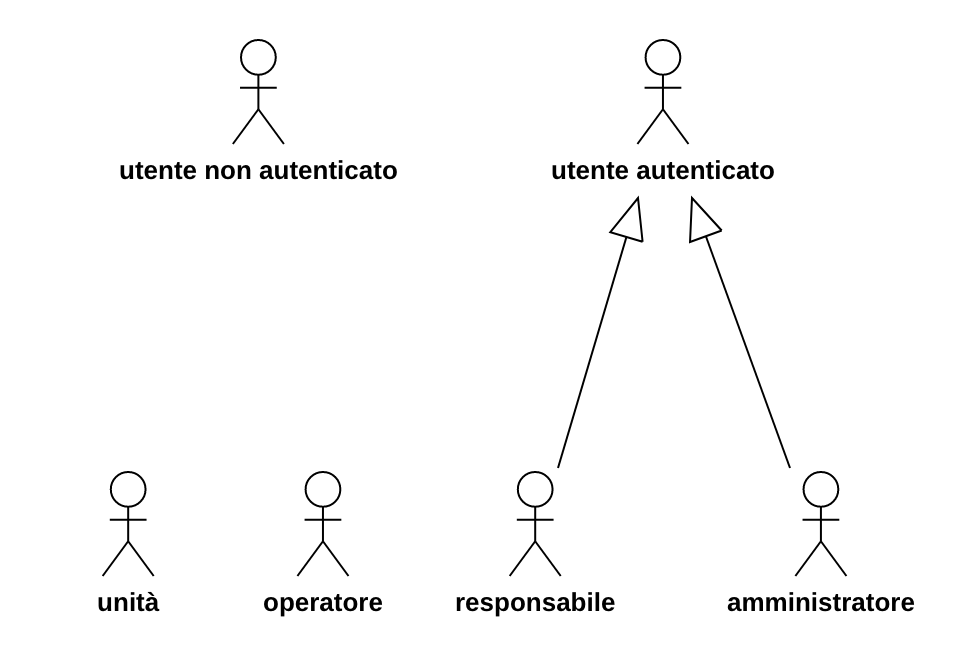
\includegraphics[scale=0.75]{res/images/gerarchia.png}
	\caption{Attori primari}
\end{figure}
\begin{itemize}
	\item{\textbf{Utente non autenticato:}\\
	Si riferisce ad un utente generico che non ha ancora effettuato l'accesso all'applicativo.}
	\item{\textbf{Utente autenticato:}\\
	Si riferisce ad un utente generico che ha effettuato l'accesso all'applicativo tramite il codice identificativo generato al momento dell'iscrizione;}
	\item{\textbf{Operatore:}\\
	Si riferisce alla persona che utilizza l'unità e si interfaccia con il sistema. Può guidare il muletto attraverso la guida manuale e controllare i movimenti effettuati dal server. Inoltre gestisce il carico e lo scarico delle merci per soddisfare ogni task che gli viene assegnata.}
	\item{\textbf{Responsabile:}\\
	 \`E la figura in capo della logistica del magazzino: inserisce le task che devono essere svolte dagli operatori.}
	\item{\textbf{Amministratore:}\\
 Ha in capo la gestione operativa: inserisce, modifica ed elimina gli account del personale per l'accesso al server, censisce i muletti nel database, crea e modifica la planimetria e la percorribilità della mappa del magazzino.}
	\item {\textbf{Unità:}\\
	Rappresenta il muletto che si muove all'interno della mappa per raggiungere i POI . }
\end{itemize}

\subsection{UC1 - Login}
\begin{figure}[H]
	\centering
	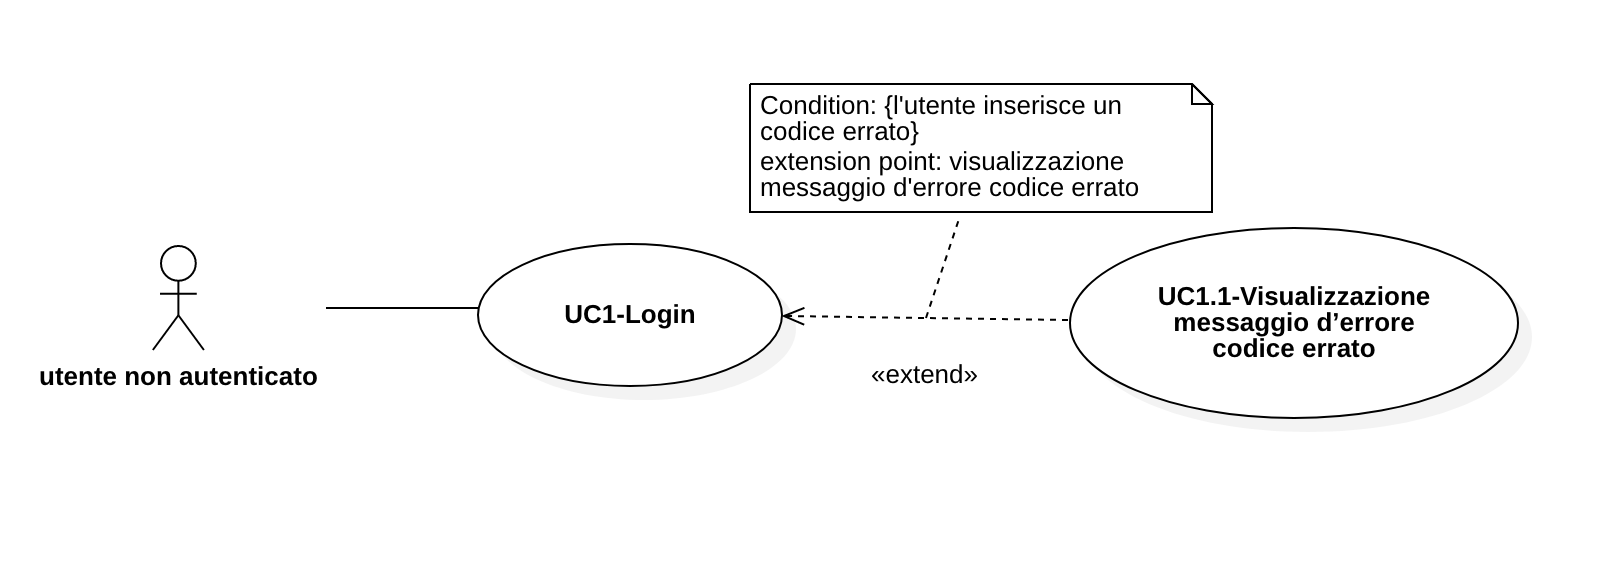
\includegraphics[scale=0.6]{res/images/uc1.PNG}
	\caption{UC1 - Login}
\end{figure}


\begin{itemize}
	\item 	\textbf{Attori primari:} utente non autenticato;
	\item 	\textbf{Precondizioni:} l'utente non è autenticato nell'applicativo;
	\item 	\textbf{Postcondizioni:}	l'utente si è autenticato con successo come amministratore o responsabile. Il server rende disponibili diverse pagine e funzionalità a seconda della tipologia di utente;
	\item 	\textbf{Scenario principale:} un utente non ancora autenticato richiede il login inserendo nell'apposito form i dati necessari, ossia codice identificativo e password. Successivamente viene confermato il login per autenticarsi. Se un codice identificato non è presente nel sistema e/o la password dello specifico codice identificativo è errata, verrà mostrato un messaggio d'errore;
	\item 	\textbf{Descrizione:} l'utente tenta di autenticarsi attraverso il suo codice personale identificativo e la sua password;
\end{itemize}

\subsubsection{UC1.1 - Inserimento codice identificativo}
\begin{itemize}
	\item \textbf{Attori primari}: utente non autenticato;
\item \textbf{Precondizioni}: l'utente non è autenticato nell'applicativo e si appresta ad iniziare il proprio lavoro;
\item \textbf{Postcondizioni}: viene visualizzato nell'apposito spazio per l'inserimento del codice identificativo, il codice identificativo immesso;
\item \textbf{Scenario principale}: l'utente, non ancora autenticato, inserisce il suo codice identificativo nell'apposito form;
\item \textbf{Descrizione}: l'utente vuole autenticarsi, inserendo il suo codice identificativo.
\end{itemize}

\subsubsection{UC1.2 - Inserimento password}
\begin{itemize}
\item \textbf{Attori primari}: utente non autenticato;
\item \textbf{Precondizioni}: l'utente non è autenticato nell'applicativo e si appresta a iniziare il proprio lavoro;
\item \textbf{Postcondizioni}: viene visualizzata nell'apposito spazio per l'inserimento della password, la password immessa oscurata;
\item \textbf{Scenario principale}: l'utente non ancora autenticato, inserisce la sua password nell'apposito input dentro il form;
\item \textbf{Descrizione}: l'utente vuole autenticarsi, inserendo la sua password.
\end{itemize}

\subsection{UC2 - Registrazione nuovo utente}

\begin{figure}[H]
	\centering
	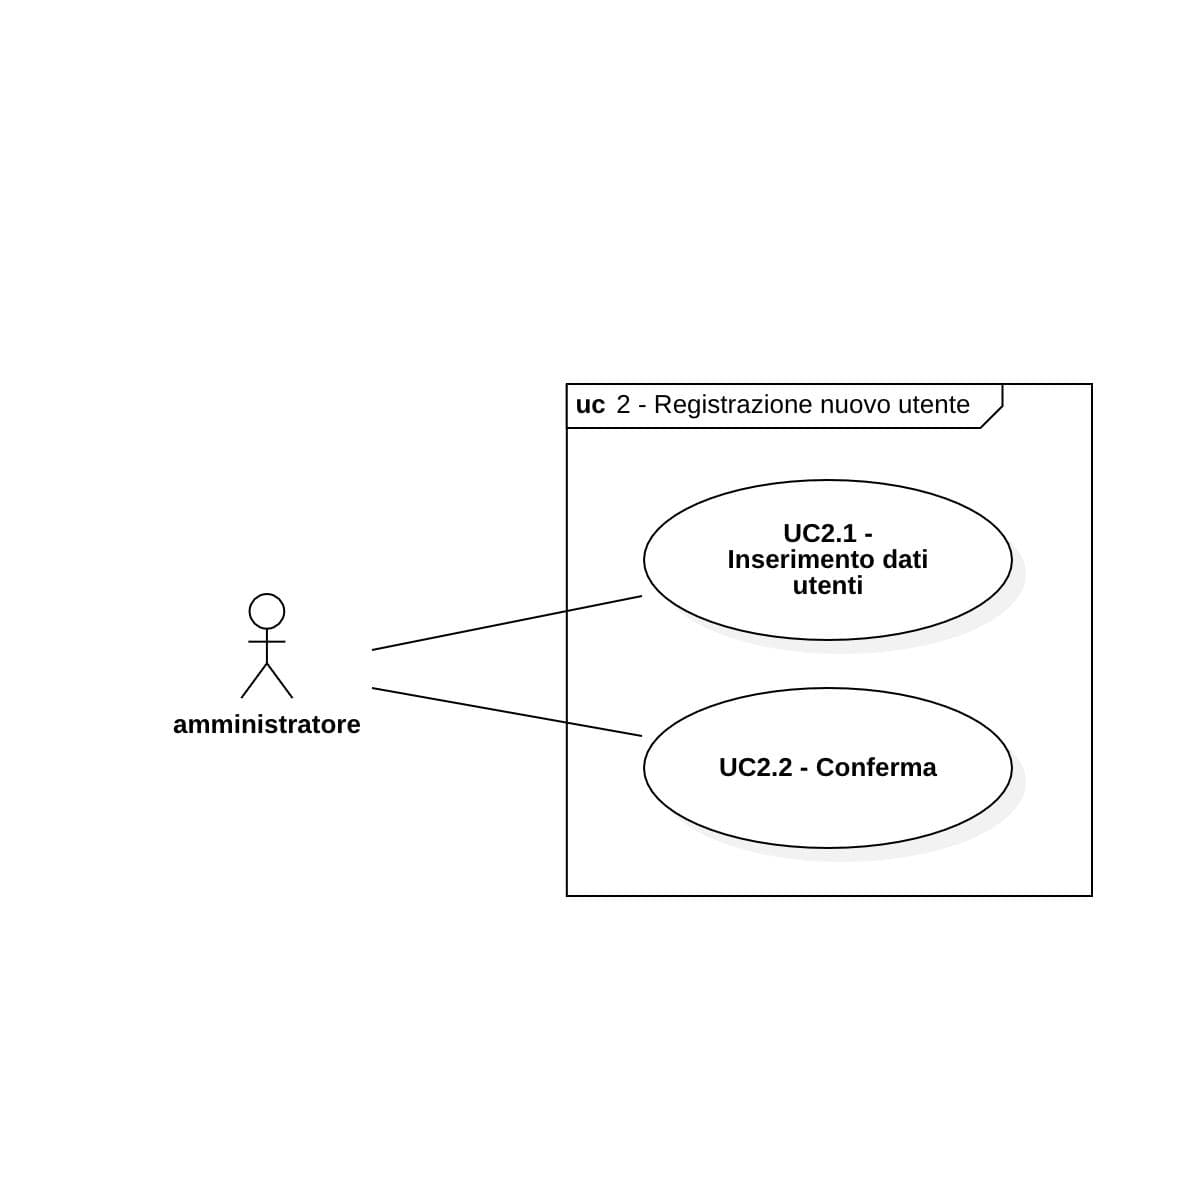
\includegraphics[scale=0.55]{res/images/uc2.png}
	\caption{UC2 - Registrazione nuovo utente}
\end{figure}
\begin{itemize}
	\item 	\textbf{Attori primari:} amministratore;
	\item 	\textbf{Precondizioni:}	l'amministratore intende inserire un nuovo responsabile assunto nell'azienda e non ancora registrato nell'applicativo.
	\item 	\textbf{Postcondizioni:} l'utente è registrato nel server correttamente come responsabile;
	\item 	\textbf{Scenario principale:} l'amministratore inserisce i dati personali del lavoratore che vuole registrare nell'applicativo;
	\item 	\textbf{Descrizione:} per effettuare l'aggiunta di un nuovo responsabile, l'amministratore deve compilare i dati dell'account che non devono essere presenti all'interno del server.

\end{itemize}

\subsubsection{UC2.1 - Inserimento dati utente}

\begin{figure}[H]
	\centering
	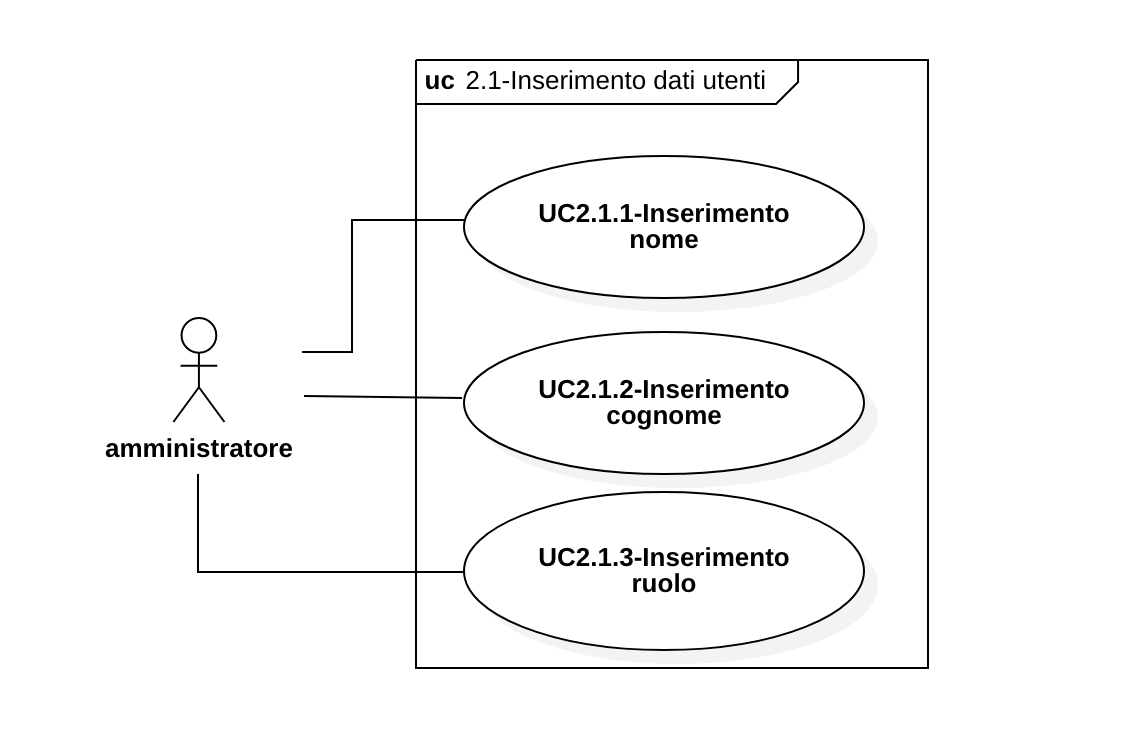
\includegraphics[scale=0.52]{res/images/uc2-1.png}
	\caption{UC2.1 - Inserimento dati utente}
\end{figure}

\begin{itemize}
	\item 	\textbf{Attori primari:} amministratore;
	\item 	\textbf{Precondizioni:}	l'amministratore sta eseguendo la registrazione del lavoratore nel server;
	\item 	\textbf{Postcondizioni:} l'amministratore ha inserito i dati in tutti i campi del form di registrazione richiesti;
	\item 	\textbf{Scenario principale:} l'amministratore compila tutti i campi del form richiesti per la registrazione, ovvero:
	\begin{itemize}
		\item inserisce il nome del lavoratore (UC2.1.1);
		\item inserisce il cognome del lavoratore (UC2.1.2);
	\end{itemize}
	\item 	\textbf{Descrizione:} per effettuare la registrazione, l'amministratore deve fornire i seguenti dati dell'utente:
	\begin{itemize}
		\item nome;
		\item cognome.
	\end{itemize}
Il server poi ritornerà un codice identificativo e una password standard, con i quali il responsabile potrà fare il primo login, per poi poter modificare la password (UC3.1.3) per averne una privata.
\end{itemize}

\paragraph{UC2.1.1 - Inserimento nome}
\begin{itemize}
	\item 	\textbf{Attori primari:} amministratore;
	\item 	\textbf{Precondizioni:} il server ha reso disponibile il campo del form per inserire il nome del lavoratore;
	\item 	\textbf{Postcondizioni:} l'amministratore ha compilato il campo con il nome;
	\item 	\textbf{Scenario principale:} l'amministratore compila il campo del form relativo al nome del lavoratore;
	\item 	\textbf{Descrizione:} per effettuare l'aggiunta di un nuovo utente, l'amministratore deve inserire il nome del lavoratore che si intende registrare.

\end{itemize}

\paragraph{UC2.1.2 - Inserimento cognome}

\begin{itemize}
	\item 	\textbf{Attori primari:} amministratore;
	\item 	\textbf{Precondizioni:} il server ha reso disponibile il campo del form per inserire il cognome del lavoratore;
	\item 	\textbf{Postcondizioni:} l'amministratore ha compilato il campo con il cognome;
	\item 	\textbf{Scenario principale:} l'amministratore compila il campo del form relativo al cognome del lavoratore;
	\item 	\textbf{Descrizione:} per effettuare l'aggiunta di un nuovo utente, l'amministratore deve inserire il cognome del lavoratore che si intende registrare.
	
\end{itemize}

\subsubsection{UC2.2 - Conferma}

\begin{itemize}
	\item 	\textbf{Attori primari:} amministratore;
	\item 	\textbf{Precondizioni:} l'amministratore ha compilato il form per l'inserimento dei dati del nuovo utente e rende disponibile un pulsante per la conferma;
	\item 	\textbf{Postcondizioni:} viene visualizzato a video un messaggio con la conferma della ricezione dei dati e il codice identificativo;
	\item 	\textbf{Scenario principale:} l'amministratore preme il pulsante di conferma dopo aver completato tutti i campi del form;
	\item 	\textbf{Descrizione:} l'amministratore preme il pulsante per la conferma dell'inserimento dei dati. A schermo viene visualizzato un messaggio con l'avvenuta registrazione e il codice identificativo relativo all'account registrato.

\end{itemize}

\subsection{UC3 - Gestione account già presenti}
\begin{figure}[H]
	\centering
	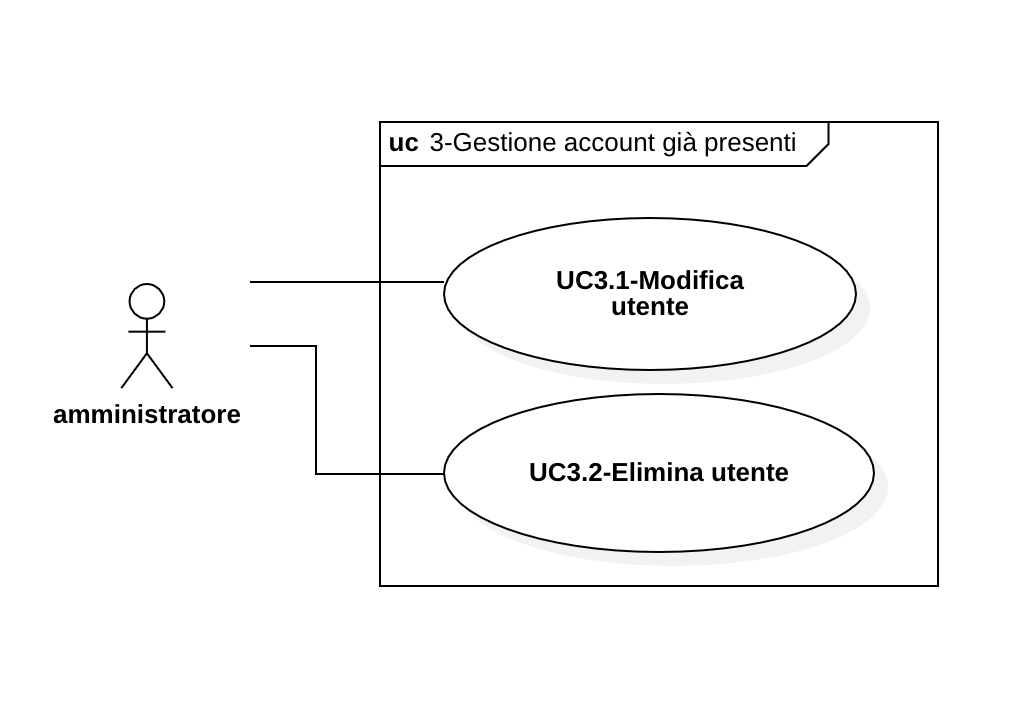
\includegraphics[scale=0.62]{res/images/uc3.png}
	\caption{UC3 - Gestione account già presenti}
\end{figure}

\begin{itemize}
	\item 	\textbf{Attori primari:} amministratore;
	\item 	\textbf{Precondizioni:} l'utente intende svolgere delle azioni su uno o più account inseriti;
	\item 	\textbf{Postcondizioni:} l'utente ha effettuato le azioni che intendeva fare (o di modifica o di eliminazione di uno o più utenti o di visualizzazione della lista di utenti inseriti);
	\item 	\textbf{Scenario principale:} 
	l'amministratore preme l'apposito pulsante per la gestione degli account presenti. Il sistema riceve la richiesta e visualizza le operazioni tra cui può scegliere, ovvero:
	\begin{itemize}
		\item UC3.1 - Modifica utente;
		\item UC3.2 - Eliminazione utente;
		\item UC3.3 - Visualizzazione lista utenti;
		\item UC3.4 - Reset password responsabile;
	\end{itemize}
	\item 	\textbf{Descrizione:} L'amministratore può gestire (e quindi modificare) i dati personali di tutti gli account registrati.
\end{itemize}

\subsubsection{UC3.1 - Modifica utente}

\begin{figure}[H]
	\centering
	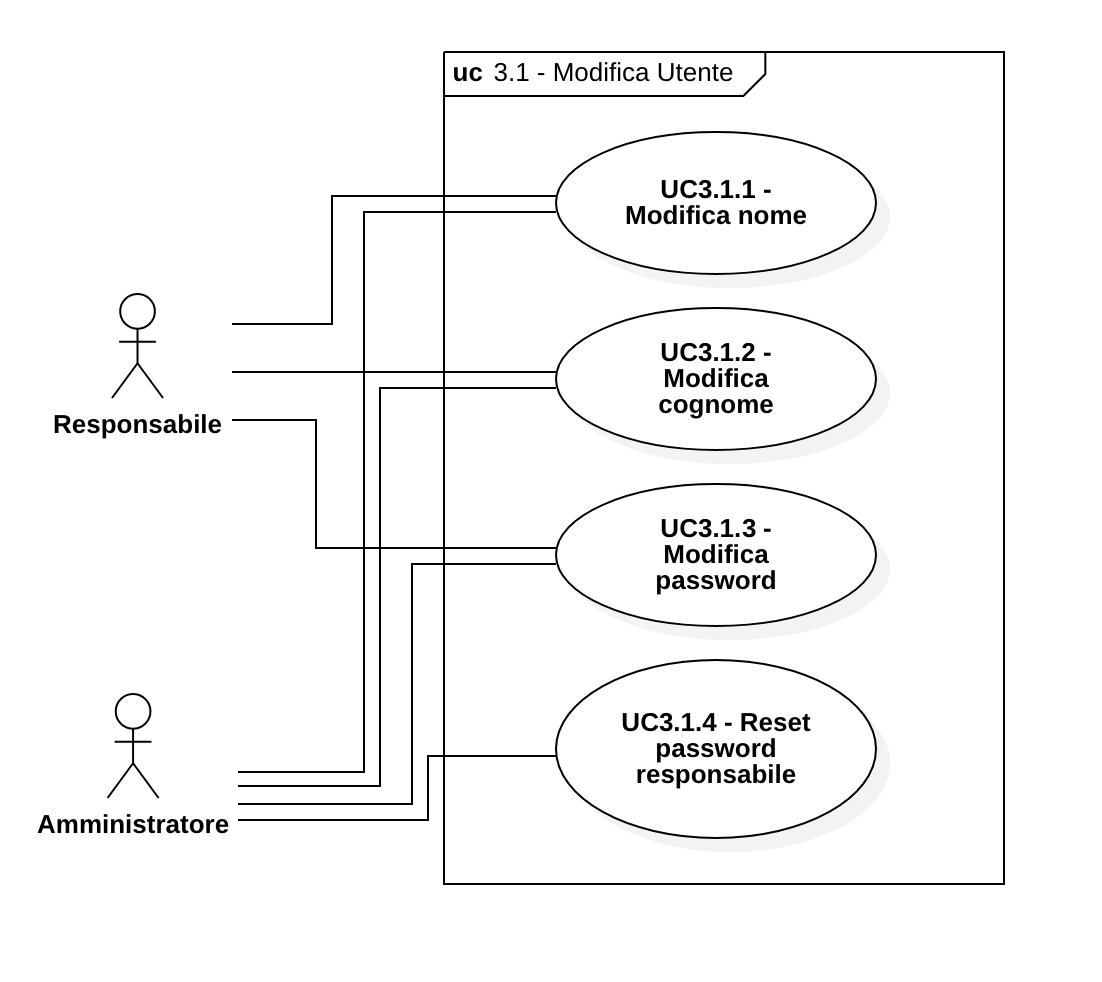
\includegraphics[scale=0.52]{res/images/uc3-1.png}
	\caption{UC3.1 - Modifica utente}
\end{figure}
\begin{itemize}
	\item 	\textbf{Attori primari:} amministratore, responsabile;
	\item 	\textbf{Precondizioni:} l'amministratore è entrato nella pagina di gestione account già presenti e premuto sul pulsante per la modifica di un utente;
	\item 	\textbf{Postcondizioni:} l'amminsitratore ha cambiato il profil di un utente;
	\item 	\textbf{Scenario principale:} l'amministratore visualizza la lista di utenti e seleziona quello che intende modificare. Il sistema visualizza i dettagli dell'account (nome, cognome) i quali possono essere modificati. In fine conferma le operazioni;
	\item 	\textbf{Descrizione:} l'amministrare vuole modificare i dati di un account.

\end{itemize}

\paragraph{UC3.1.1 - Modifica nome}

\begin{itemize}
	\item 	\textbf{Attori primari:} amministratore, responsabile;
	\item 	\textbf{Precondizioni:} è stato reso disponibile il campo per la modifica del nome utente;
	\item 	\textbf{Postcondizioni:}  l'utente ha compilato il campo con il nome aggiornato;
	\item 	\textbf{Scenario principale:} l'utente compila il campo del form per aggiornare il nome;
	\item 	\textbf{Descrizione:} per effettuare la modifica del campo relativo al nome, l'utente aggiorna il valore nel form.
\end{itemize}

\paragraph{UC3.1.2 - Modifica cognome}

\begin{itemize}
	\item 	\textbf{Attori primari:} amministratore, responsabile;
	\item 	\textbf{Precondizioni:} è stato reso disponibile il campo per la modifica del cognome utente;
	\item 	\textbf{Postcondizioni:} l'utente ha compilato il campo con il cognome aggiornato;
	\item 	\textbf{Scenario principale:} l'utente compila il campo del form relativo al cognome da aggiornare;
	\item 	\textbf{Descrizione:} per effettuare la modifica del campo relativo al cognome, l'utente aggiorna il valore nel form.

\end{itemize}


\subsubsection{UC3.2 - Elimina utente}

\begin{itemize}
	\item 	\textbf{Attori primari:} amministratore;
	\item 	\textbf{Precondizioni:} l'amministratore ha premuto l'apposito pulsante per l'eliminazione di un utente;
	\item 	\textbf{Postcondizioni:} è stato eliminato dal server l'account dell'utente selezionato;
	\item 	\textbf{Scenario principale:} l'amministratore visualizza la lista di tutti gli utenti registrati nel sistema. Seleziona l'account desiderato, il sistema visualizza un messaggio di conferma per l'eliminazione. L'attore quindi conferma tramite l'apposito bottone; 
	\item 	\textbf{Descrizione:} può essere necessario eliminare l'account di un utente.
\end{itemize}

\subsubsection{UC3.3 - Visualizzazione lista utenti}

\begin{itemize}
	\item 	\textbf{Attori primari:} amministratore;
	\item 	\textbf{Precondizioni:} l'amministratore vuole vedere la lista dei responsabili presenti nel server;
	\item 	\textbf{Postcondizioni:} l'amministratore preme l'apposito pulsante per la visualizzazione della lista di utenti;
	\item 	\textbf{Scenario principale:} l'amministratore visualizza l'intera lista di utenti;
	\item 	\textbf{Descrizione:} può essere necessario da parte dell'amministratore, visualizzare la lista di tutti i responsabili inseriti e i loro relativi dati pubblici.
\end{itemize}

\paragraph{UC3.4 - Reset password responsabile}

\begin{itemize}
	\item 	\textbf{Attori primari:} amministratore;
	\item 	\textbf{Precondizioni:} l'amministratore ha premuto il pulsante per il reset password;
	\item 	\textbf{Postcondizioni:} viene resettata la password di un responsabile e viene visualizzata a video la nuova password di default;
	\item 	\textbf{Scenario principale:} l'amministratore visualizza la lista completa di responsabili. Seleziona l'utente desiderato. Il sistema viene notificato e rielabora una nuova password che poi stampa a video all'amministratore;
	\item 	\textbf{Descrizione:} un responsabile può perdere o dimenticare la propria password di accesso. L'amministratore quindi dovrà aver a disposizione un sistema che permetta di resettare la password di un certo responsabile.

\end{itemize}

\subsection{UC4 - Gestione task}

\begin{figure}[H]
	\centering
	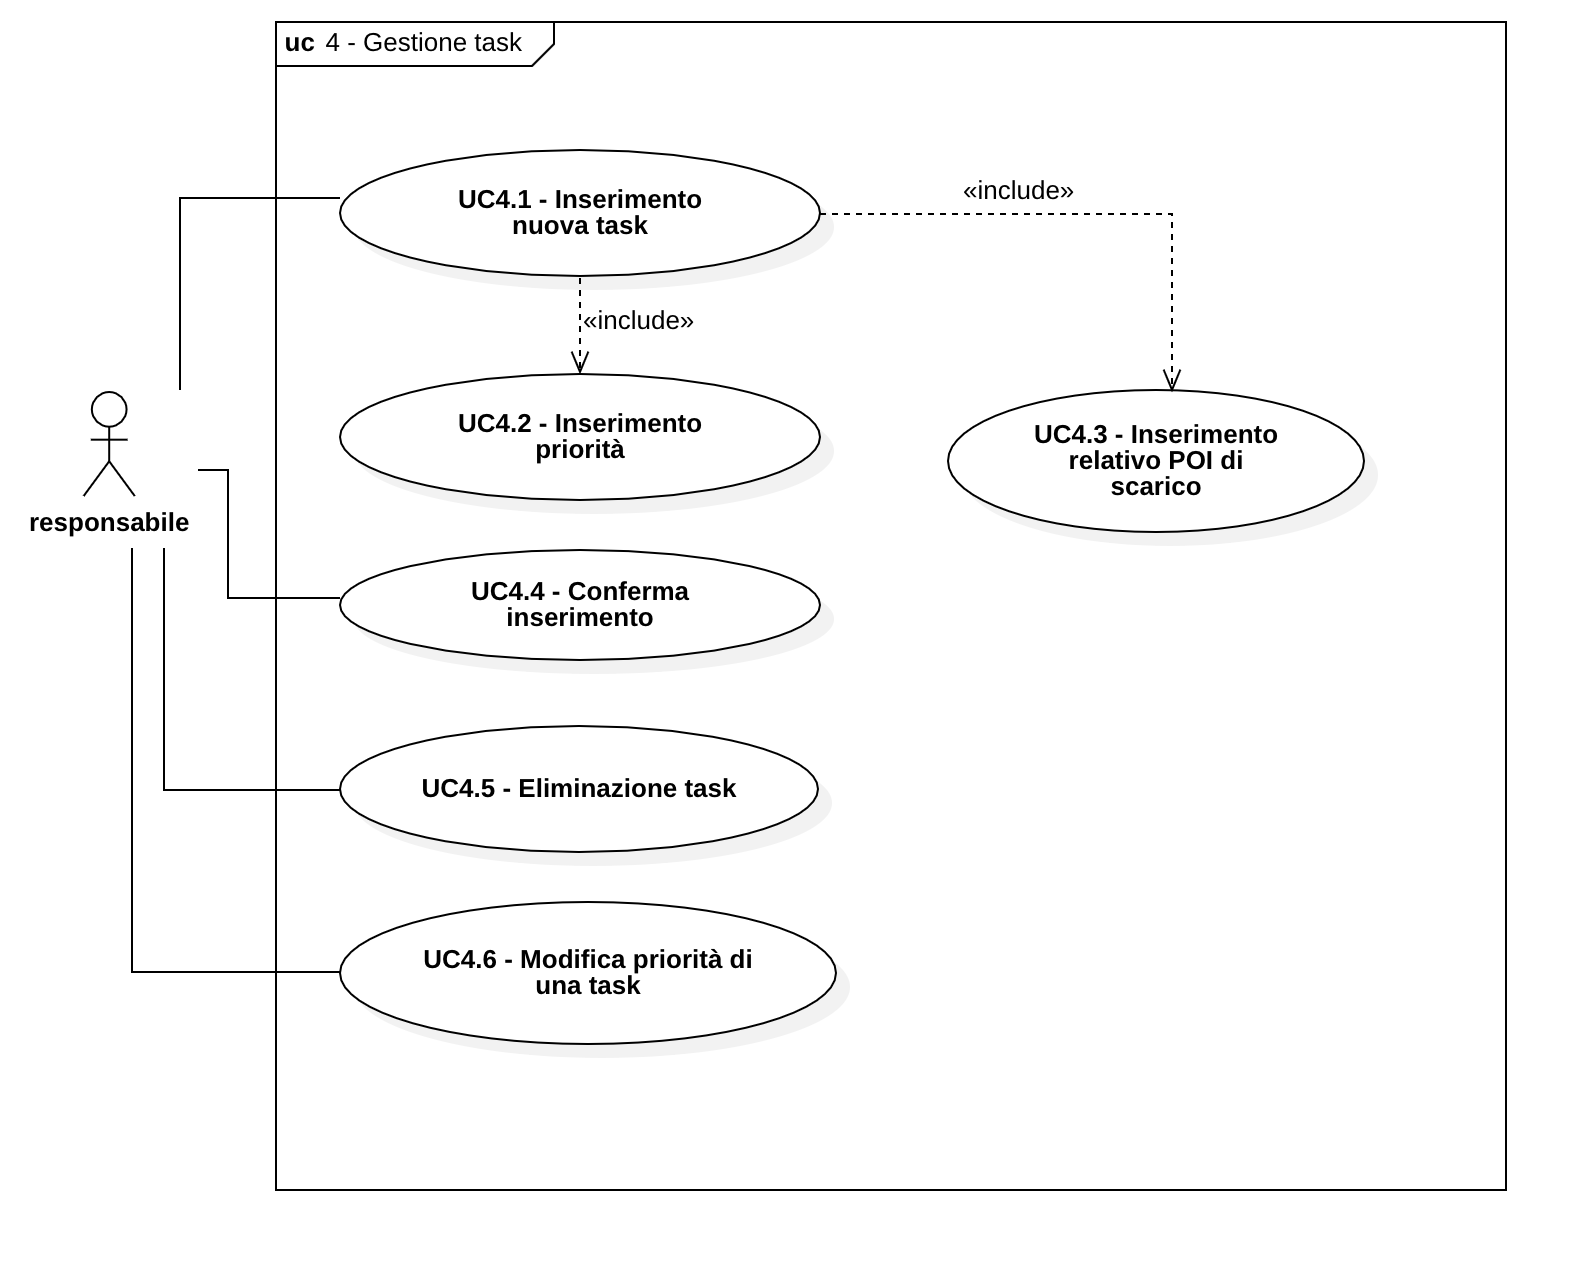
\includegraphics[scale=0.52]{res/images/uc4.png}
	\caption{UC4 - Gestione task}
\end{figure}

\begin{itemize}
	\item 	\textbf{Attori primari:} responsabile;
	\item 	\textbf{Precondizioni:} il responsabile è autenticato nel sistema il quale rende disponibile l'interfaccia per la gestione delle task che verranno assegnate alle unità;
	\item 	\textbf{Postcondizioni:} la lista di task viene aggiornata;
	\item 	\textbf{Scenario principale:} il responsabile effettua le operazioni necessarie per la gestione delle task da far soddisfare alle unità, esse possono essere:
	\begin{itemize}
		\item l'inserimento di una nuova lista ordinata di task (UC4.1) che verrà poi assegnata dal sistema ad un'unità;
		\item l'eliminazione di una lista di task già creata precedentemente (UC4.2);
	\end{itemize}
	\item 	\textbf{Descrizione:} lo scarico delle merci in un determinato punto di interesse di scarico viene chiamato task\textsubscript{G}. Il responsabile inserisce delle liste di task ordinate che verranno assegnate dal sistema ad ogni unità. 

\end{itemize}

\subsubsection{UC4.1 - Inserimento nuova lista ordinata di task}

\begin{figure}[H]
	\centering
	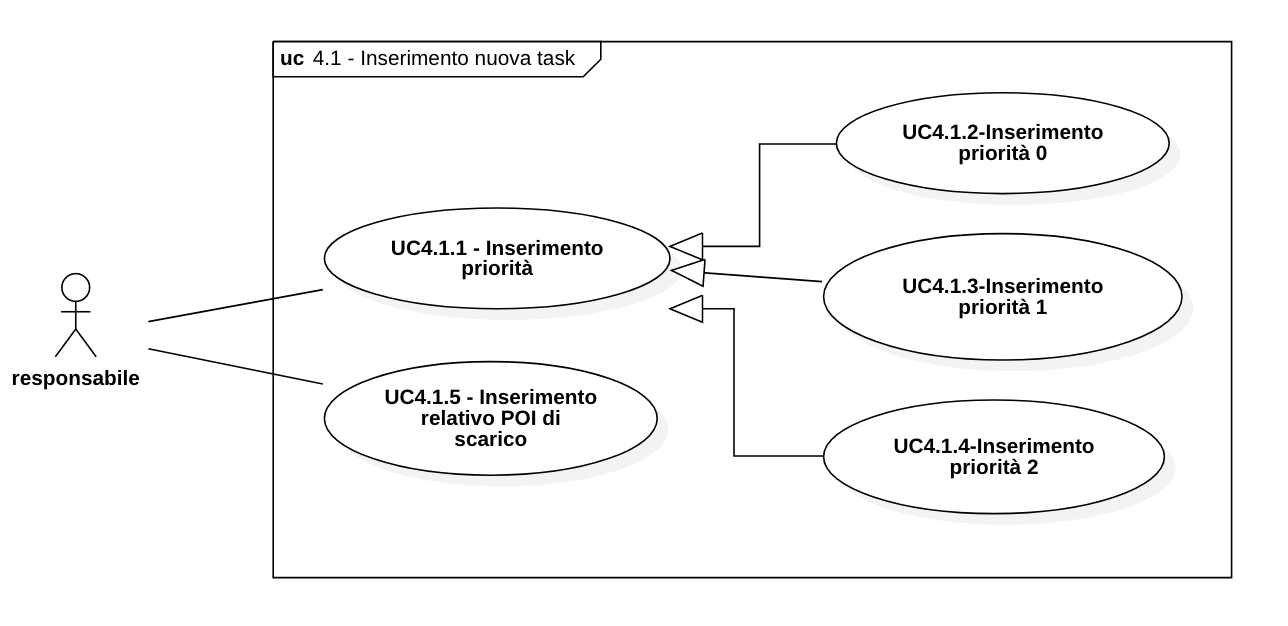
\includegraphics[scale=0.52]{res/images/uc4-1.png}
	\caption{UC4.1 - Inserimento nuova task}
\end{figure}

\begin{itemize}
	\item 	\textbf{Attori primari:} responsabile;
	\item 	\textbf{Precondizioni:} è resa disponibile l'interfaccia per l'inserimento di una nuova lista di task\textsubscript{G}; 
	\item 	\textbf{Postcondizioni:} il responsabile ha aggiunto con successo una nuova lista di task ordinata che verrà assegnata ad un'unità, la quale la visualizzerà nella propria lista di compiti (UC8);
	\item 	\textbf{Scenario principale:} il responsabile preme l'apposito pulsante per l'aggiunta di una nuova lista di task\textsubscript{G} e visualizza le operazioni che può intraprendere per creare questa nuova lista, ossia:
	\begin{itemize}
		\item l'aggiunta di una task singola con il proprio POI di scarico per soddisfarla (UC4.1.1);
		\item la rimozione di una task già aggiunta nella lista che si sta creando (UC4.1.2);
		\item la conferma della lista che si è creata, così che il sistema la possa prendere in carico (UC4.1.3);
	\end{itemize}
	\item 	\textbf{Descrizione:} i compiti da svolgere sono organizzati in liste di task ordinate, ognuna assegnata ad un'unità che dovrà soddisfarla. Il responsabile ha il compito di creare ogni lista che verrà gestita dal sistema.
\end{itemize}

\paragraph{UC4.1.1 - Aggiunta nuova task alla lista}
\begin{itemize}
	\item 	\textbf{Attori primari:} responsabile;
	\item 	\textbf{Precondizioni:} il responsabile sta creando una nuova lista di task;
	\item 	\textbf{Postcondizioni:} è stata inserita alla lista corrente una nuova task;
	\item 	\textbf{Scenario principale:} il responsabile preme un apposito pulsante per l'aggiunta di una nuova task alla lista che si sta creando. Il sistema farà apparire la lista di POI di scarico dal quale selezionerà il relativo punto per soddisfare tale compito. Successivamente conferma la creazione.
	\item 	\textbf{Descrizione:} il responsabile inserisce il nuovo compito da eseguire nella lista ordinata di task che sta creando, inserendo il POI di scarico relativo dove avverrà lo scarico delle merci da parte dell'unità.
	
\end{itemize}

\paragraph{UC4.1.2 - Rimozione task dalla lista}
\begin{itemize}
	\item 	\textbf{Attori primari:} responsabile;
	\item 	\textbf{Precondizioni:} il responsabile sta creando la lista ordinata e ha aggiunto almeno una task;
	\item 	\textbf{Postcondizioni:} è stata eliminata una task dalla lista che si sta creando;
	\item 	\textbf{Scenario principale:} il responsabile preme un pulsante di eliminazione a fianco della task interessata;
	\item 	\textbf{Descrizione:} durante la creazione della lista ordinata, il responsabile deve poter rimediare ad aggiunte errate eliminando determinate task.
\end{itemize}
\paragraph{UC4.1.3 - Conferma inserimento lista}
\begin{itemize}
	\item 	\textbf{Attori primari:} responsabile;
	\item 	\textbf{Precondizioni:} il responsabile ha completato la creazione di una lista ordinata di task;
	\item 	\textbf{Postcondizioni:} la lista viene inviata al sistema che la assegnerà ad un'unità;
	\item 	\textbf{Scenario principale:} il responsabile preme l'apposito pulsante di conferma per completare la creazione della lista ordinata;
	\item 	\textbf{Descrizione:} una volta che il responsabile ha finito di creare la lista aggiungendo tutte le task che un'unità deve soddisfare, serve che confermi l'inserimento cosicché il sistema la possa gestire.
	
\end{itemize}


\subsubsection{UC4.2 - Eliminazione lista di task}

\begin{itemize}
	\item 	\textbf{Attori primari:} responsabile;
	\item 	\textbf{Precondizioni:} il responsabile visualizza le liste di task non ancora prese in carico; si accorge che una di queste non è più necessaria;
	\item 	\textbf{Postcondizioni:} è stata eliminata una lista di task da quelle non ancora prese in carico;
	\item 	\textbf{Scenario principale:} il responsabile seleziona una lista di task tra quelle non ancora prese in carico (UC13.1) e tramite un apposito bottone la elimina; il sistema quindi cancellerà dallo storico la lista e di conseguenza non l'assegnerà a nessun muletto;
	\item 	\textbf{Descrizione:} il responsabile ha inserito una lista ordinata di task errata o che non è più necessaria soddisfare, per cui intende eliminarla. Questa operazione è possibile solamente se la lista non è ancora stata presa in carico da nessuna unità.
\end{itemize}


\subsection{UC5 - Logout}

\begin{itemize}
	\item 	\textbf{Attori primari:} utente autenticato;
	\item 	\textbf{Precondizioni:} l'utente ha finito il proprio turno e il sistema visualizza il bottone di logout;
	\item 	\textbf{Postcondizioni:} l'utente viene disconnesso dal sistema;
	\item 	\textbf{Scenario principale:} l'utente preme l'apposito bottone di logout per disconnettersi dall'applicativo;
	\item 	\textbf{Descrizione:} l'utente (amministratore o responsabile) vuole effettuare il logout dall'applicativo
\end{itemize}


\subsection{UC6 - Visualizzazione mappa}

\begin{figure}[H]
	\centering
	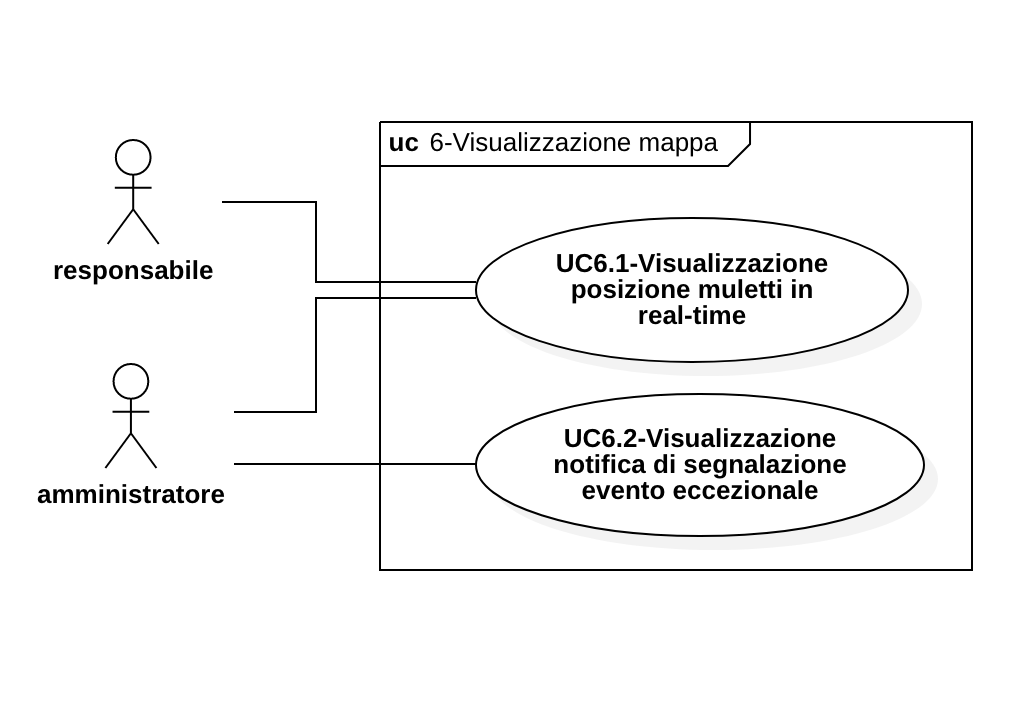
\includegraphics[scale=0.52]{res/images/uc6.png}
	\caption{UC6 - Visualizzazione mappa}
\end{figure}

\begin{itemize}
	\item 	\textbf{Attori primari:} amministratore, responsabile;
	\item 	\textbf{Precondizioni:} gli attori sono autenticati nel sistema;
	\item 	\textbf{Postcondizioni:} gli attori visualizzano la mappa del magazzino;
	\item 	\textbf{Scenario principale:} il responsabile e l'amministratore, una volta autenticati, visualizzano la mappa completa del magazzino;
	\item 	\textbf{Descrizione:} il responsabile e l'amministratore supervisionano il magazzino tramite una mappa che ne visualizza gli elementi strutturali. Gli elementi della mappa sono:
	\begin{itemize}
		\item POI di carico:  punto in cui i muletti prelevano il carico di merce da smistare nel magazzino. Ogni volta che completano la loro lista di task (ma non è finito il loro turno di lavoro), devono tornare su questo punto per effettuare un nuovo carico e ricevere nuove task\textsubscript{G};
		\item POI di scarico: punti in cui i muletti devono scaricare la merce prelevata;
		\item POI di sosta o di base: punto in cui gli operatori partono con il proprio muletto a inizio turno e arrivano alla fine del turno;
		\item zona di percorrenza\textsubscript{G}: strade in cui i muletti possono transitare, caratterizzata dal senso di marcia;
		\item aree non transitabili: muri, scaffali, elementi e zone del magazzino che non prevedono il transito di un muletto.
	\end{itemize}

\end{itemize}


\subsubsection{UC6.1 - Visualizzazione posizione muletti in real-time}
\begin{itemize}
	\item 	\textbf{Attori primari:} amministratore, responsabile;
	\item 	\textbf{Precondizioni:} gli attori sono autenticati nel sistema e visualizzano correttamente la mappa;
	\item 	\textbf{Postcondizioni:} gli attori visualizzano gli spostamenti dei muletti in real-time nella mappa;
	\item 	\textbf{Scenario principale:} il responsabile e l'amministratore una volta autenticati, visualizzano la mappa completa del magazzino con i muletti in movimento;
	\item 	\textbf{Descrizione:} il responsabile e l'amministratore supervisionano il magazzino tramite una mappa che visualizza in real-time la posizione dei muletti al suo interno.
\end{itemize}

\subsubsection{UC6.2 - Visualizzazione notifica di segnalazione evento eccezionale}
\begin{itemize}
	\item 	\textbf{Attori primari:} amministratore;
	\item 	\textbf{Precondizioni:} è stato segnalato un evento eccezionale da un operatore;
	\item 	\textbf{Postcondizioni:} viene visualizzata una notifica che avverte l'amministratore dell'avvenimento un evento eccezionale;
	\item 	\textbf{Scenario principale:} il sistema visualizza una notifica di segnalazione dell'avvenimento di un evento eccezionale, evidenziando il punto in cui si è verificato;
	\item 	\textbf{Descrizione:} l'operatore mentre sta completando le proprie task\textsubscript{G}, può segnalare l'avvenimento di un evento eccezionale all'interno del magazzino (UC11.3). Il sistema dovrà notificare l'amministratore di questo e indicargli la posizione in cui è stato riscontrato.
\end{itemize}

\subsection{UC7 - Modifica mappa}



\begin{figure}[H]

   \centering

   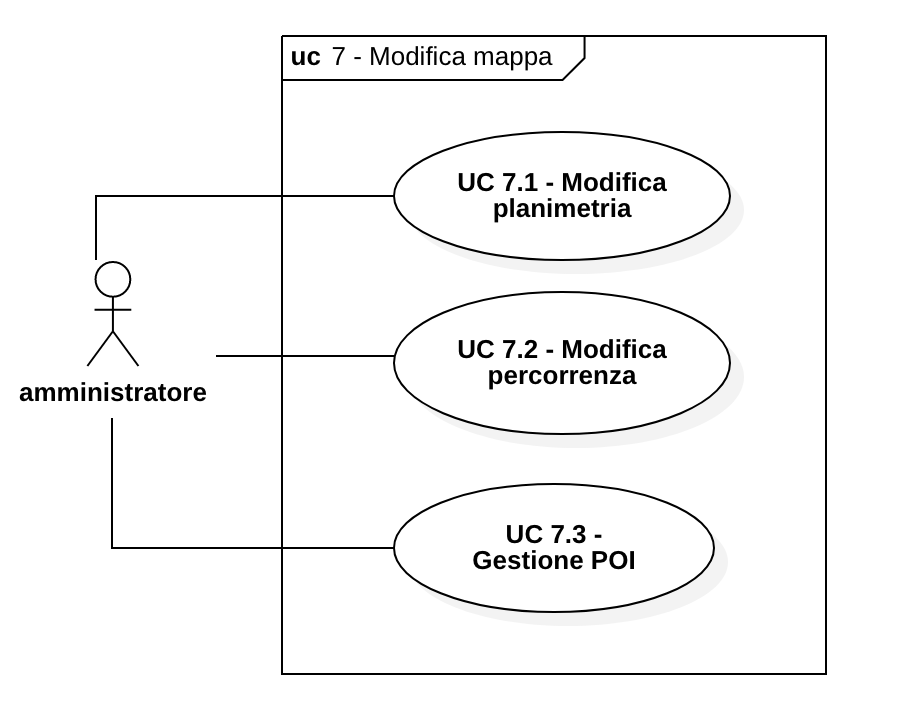
\includegraphics[scale=0.52]{res/images/uc7.png}

  \caption{UC7 - Gestione mappa}

\end{figure}



\begin{itemize}

   \item   \textbf{Attori primari} amministratore;

  \item   \textbf{Precondizioni:} viene resa disponibile dal sistema l'interfaccia per la modifica della mappa;

   \item   \textbf{Postcondizioni:} la mappa è stata modificata dall'amministratore;

  \item   \textbf{Scenario principale:} l'amministratore dopo aver premuto il pulsante per la modifica, visualizza l'interfaccia per gestire i cambiamenti della mappa tra cui può scegliere tramite un menù a tendina se:

   \begin{itemize}
     \item modificare la planimetria del magazzino (UC7.1);

      \item modificare la percorrenza del magazzino, per esempio i sensi di marcia (UC7.2);

      \item gestire i POI (UC7.3);
  \end{itemize}

  e viene visualizzata l'intera mappa (UC6).

Terminata la modifica, l'amministratore salva tramite l'apposito pulsante di conferma;

 \item   \textbf{Descrizione:} l'amministratore ha il compito di tenere aggiornata la mappa dai cambiamenti reali del magazzino, modificandone la planimetria\textsubscript{G}, la percorrenza e i POI presenti.

\end{itemize}





\subsubsection{UC7.1 - Modifica planimetria}

\begin{itemize}

  \item   \textbf{Attori primari:} amministratore;

  \item   \textbf{Precondizioni:} viene resa disponibile dal sistema l'interfaccia per la modifica della planimetria della mappa; nessuna unità deve circolare al momento della modifica;

 \item   \textbf{Postcondizioni:} la mappa è stata modificata dall'amministratore;

 \item   \textbf{Scenario principale:} vengono visualizzati degli strumenti per la modifica della planimetria\textsubscript{G}:

 \begin{itemize}

      \item ampliamento;

    \item riduzione;
      \item aggiunta, rimozione e modifica zone non transitabili.

  \end{itemize}

  Una volta raggiunto il risultato desiderato, l'amministratore conferma tramite il pulsante di salvataggio;

  \item   \textbf{Descrizione:} il magazzino, con il passare del tempo, può subire dei cambiamenti nella planimetria\textsubscript{G}. Possono venire modificati:

\begin{itemize}

     \item la dimensione del magazzino (ampliarlo o diminuirlo);
     \item le zone in cui non è permessa la transizione dei mezzi (scaffali, muri, elementi e zone del magazzino che non prevedono il transito di un muletto).

  \end{itemize}

\end{itemize}



\subsubsection{UC7.2 - Modifica percorrenza}

\begin{itemize}

  \item   \textbf{Attori primari:} amministratore;

  \item   \textbf{Precondizioni:}  l'amministratore è autenticato nel sistema e viene reso disponibile dal sistema l'interfaccia per la modifica della percorrenza della mappa; nessuna unità deve circolare nell'area selezionata per il cambiamento;

  \item   \textbf{Postcondizioni:} la mappa è stata modificata dall'amministratore;
 \item   \textbf{Scenario principale:} viene visualizzata la mappa con il senso di marcia per ogni area di percorrenza. L'amministratore deve premere sopra la zona che intende cambiare per aprire un pop-up e inserire gli aggiornamenti. Una volta raggiunto il risultato desiderato, l'amministratore conferma tramite il pulsante di salvataggio;

  \item   \textbf{Descrizione:} il magazzino può subire dei cambiamenti nella percorrenza\textsubscript{G}. Sarà possibile modificare per ogni area il senso di marcia.

\end{itemize}



\subsubsection{UC7.3 - Gestione POI}



\begin{figure}[H]

 \centering

 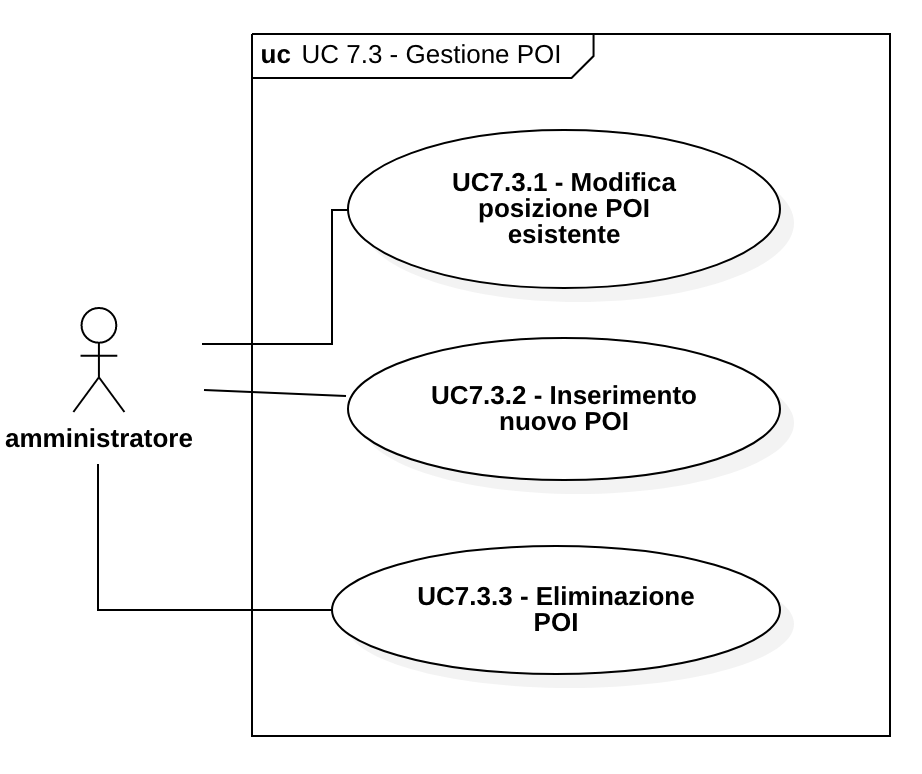
\includegraphics[scale=0.52]{res/images/uc7-3.png}

 \caption{UC7.3 - Gestione POI}

\end{figure}



\begin{itemize}

\item   \textbf{Attori primari:} amministratore;

 \item   \textbf{Precondizioni:} l'amministratore è autenticato nel sistema e viene reso disponibile dal sistema l'interfaccia per la modifica dei POI\textsubscript{A};

 \item   \textbf{Postcondizioni:} nella mappa sono comparsi i cambiamenti dei POI\textsubscript{A}; 

\item   \textbf{Scenario principale:} l'amministratore dopo aver premuto il pulsante per la modifica dei POI\textsubscript{A}, visualizza le opzioni tra cui può scegliere le operazioni da eseguire:

  \begin{itemize}

    \item modificare la posizione di un POI esistente (UC7.3.1);

    \item aggiungere un nuovo POI nella mappa (UC7.3.2);

   \item eliminare un POI esistente (UC7.3.3).

 \end{itemize}

\item   \textbf{Descrizione:} è possibile che sia necessaria la modifica dei punti di interesse nella mappa, l'amministratore ha appunto il compito di aggiungerne, modificarne o eliminarli in base alle esigenze del magazzino. Il responsabile deve tenere presente i vincoli del magazzino altrimenti non sarà permessa l'operazione:

  \begin{itemize}

\item deve esserci almeno una base;

\item deve esserci almeno un POI di carico.

\end{itemize}

\end{itemize}



\paragraph{UC7.3.1 - Modifica posizione di un POI esistente}



\begin{itemize}

\item   \textbf{Attori primari:} amministratore;

\item   \textbf{Precondizioni:} l'amministratore ha selezionato l'opzione tra il menu della modifica dei POI per il cambiamento della posizione di un POI esistente; nessuna unità si trova nel POI selezionato;

 \item   \textbf{Postcondizioni:} il POI selezionato ha cambiato posizione nella mappa; 

\item   \textbf{Scenario principale:} l'amministratore dopo aver premuto il pulsante per la modifica della posizione di un POI esistente, visualizza la mappa (UC6) con tutti i POI nella loro posizione, seleziona quello che gli interessa e lo sposta nella posizione aggiornata;
   \item   \textbf{Descrizione:} l'amministratore può dover cambiare la posizione di alcuni POI già esistenti all'interno del magazzino.

\end{itemize}



\paragraph{UC7.3.2 - Inserimento nuovo POI}

\begin{figure}[H]

  \centering

   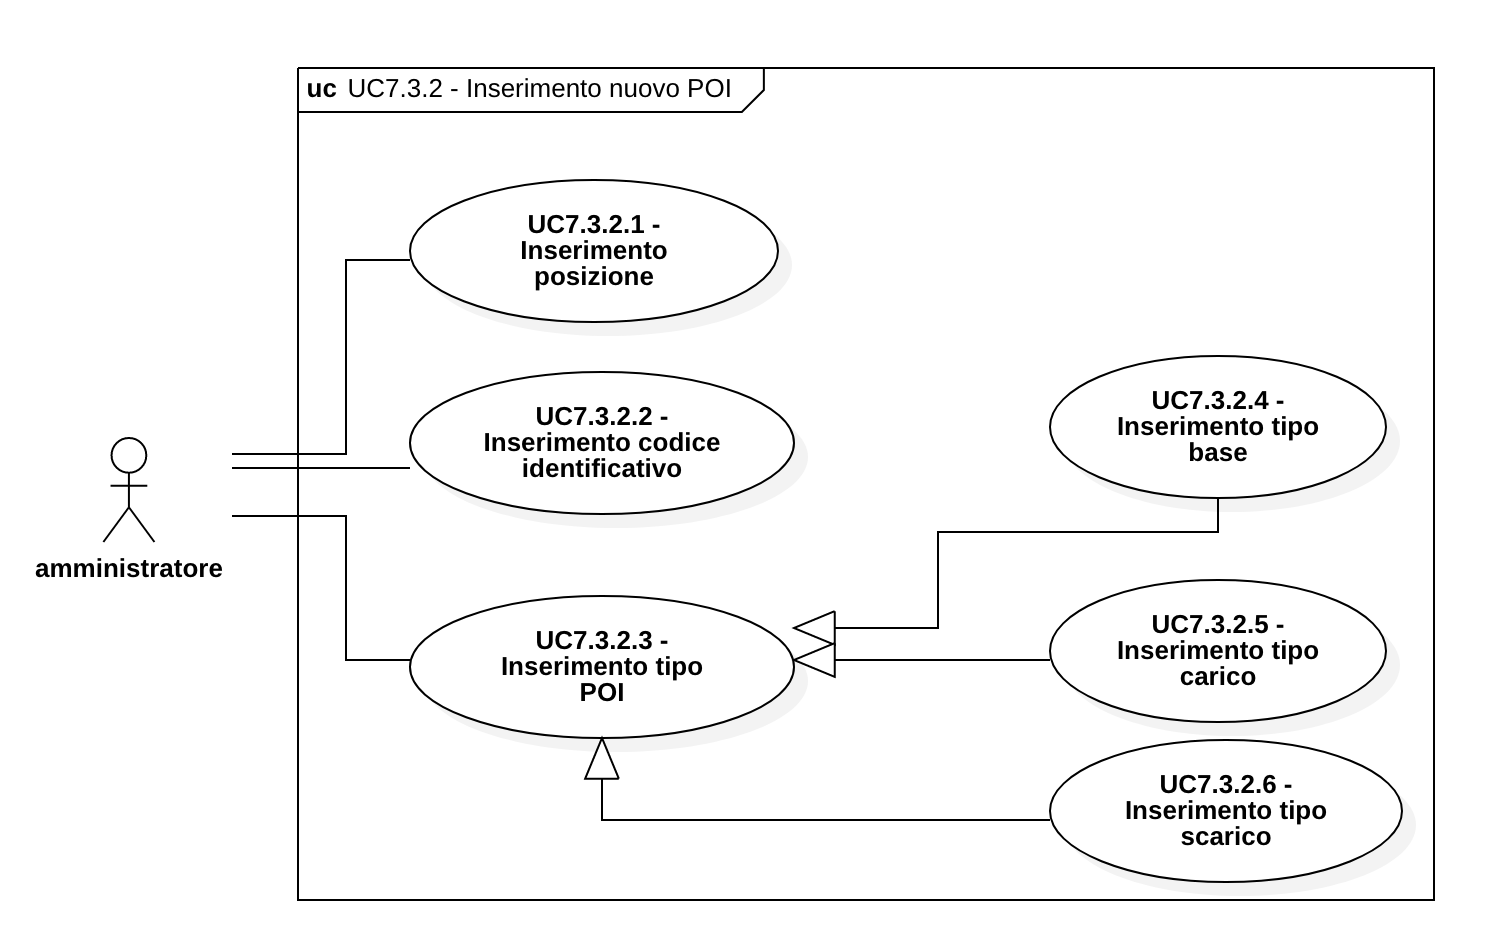
\includegraphics[scale=0.52]{res/images/uc7-3-2.png}

  \caption{UC7.3.2 - Inserimento nuovo POI}

\end{figure}



\begin{itemize}

   \item   \textbf{Attori primari:} amministratore;

   \item   \textbf{Precondizioni:} l'amministratore ha selezionato l'opzione, tra il menu, dell'aggiunta di un nuovo POI\textsubscript{A};

  \item   \textbf{Postcondizioni:} viene creato il nuovo POI nella mappa;

   \item   \textbf{Scenario principale:} l'amministratore dopo aver premuto il pulsante per l'aggiunta di un nuovo POI\textsubscript{A}, visualizzerà l'interfaccia per la creazione del nuovo punto d'interesse;

  \item   \textbf{Descrizione:} per inserire un nuovo POI all'interno della mappa devono essere specificati:

  \begin{itemize}

       \item codice identificativo;

       \item posizione nella mappa;

       \item tipo di POI (carico, scarico, base);

   \end{itemize}

\end{itemize}



\subparagraph{UC7.3.2.1 - Inserimento posizione}

\begin{itemize}

   \item   \textbf{Attori primari:} amministratore;

\item   \textbf{Precondizioni:} l'amministratore visualizza la mappa per l'inserimento dei dati del nuovo POI\textsubscript{A}.

  \item   \textbf{Postcondizioni:} l'amministratore ha inserito il POI all'interno della mappa; 

   \item   \textbf{Scenario principale:}

    \begin{itemize}
        \item visualizza la mappa (UC6);

        \item preme nel punto in cui vuole inserire il POI\textsubscript{A};
		     \item conferma l'inserimento premendo un pulsante apposito;

   \end{itemize}

   \item   \textbf{Descrizione:} per completare l'aggiunta, l'amministratore deve posizionare il POI nella mappa.



\end{itemize}



\subparagraph{UC7.3.2.2 - Inserimento codice identificativo}

\begin{itemize}

  \item   \textbf{Attori primari:} amministratore;

   \item   \textbf{Precondizioni:} l'amministratore visualizza il form per l'inserimento del codice identificativo del nuovo POI\textsubscript{A};

   \item   \textbf{Postcondizioni:} l'amministratore ha inserito il codice identificativo del nuovo POI\textsubscript{A}; 

   \item   \textbf{Scenario principale:} l'amministratore inserisce il codice identificativo del nuovo POI nell'apposito form;

   \item   \textbf{Descrizione:} per completare l'aggiunta, l'amministratore deve assegnare un codice identificativo al nuovo POI\textsubscript{A}.



\end{itemize}



\subparagraph{UC7.3.2.3 - Inserimento tipo POI}

\begin{itemize}

   \item   \textbf{Attori primari:} amministratore;

  \item   \textbf{Precondizioni:} l'amministratore visualizza il form per l'inserimento del tipo di POI\textsubscript{A};

   \item   \textbf{Postcondizioni:} viene creato il nuovo POI nella mappa; 

  \item   \textbf{Scenario principale:} l'amministratore inserisce il tipo di POI e conferma;

   \item   \textbf{Descrizione:} per completare l'aggiunta, l'amministratore deve assegnare il tipo di POI nella mappa:

  \begin{itemize}

       \item scarico;

       \item carico;

       \item base.
   \end{itemize}

   \item   \textsc{Specializzazione:}

   \begin{itemize}

       \item UC7.3.2.4 - Inserimento tipo base;

       \item UC7.3.2.5 - Inserimento tipo carico;

       \item UC7.3.2.6 - Inserimento tipo scarico;

   \end{itemize}



\end{itemize}



\subparagraph{UC7.3.2.4 - Inserimento tipo base}

\begin{itemize}

   \item   \textbf{Attori primari:} amministratore;

   \item   \textbf{Precondizioni:} l'amministratore visualizza il form per l'inserimento del tipo di POI\textsubscript{A};

   \item   \textbf{Postcondizioni:} viene creato il nuovo POI nella mappa di tipo base; 

   \item   \textbf{Scenario principale:} l'amministratore assegna al POI il tipo base;

   \item   \textbf{Descrizione:} per completare l'aggiunta, l'amministratore deve assegnare il tipo di POI nella mappa. Un POI di base è il punto in cui un'unità inizia il proprio turno.



\end{itemize}



\subparagraph{UC7.3.2.5 - Inserimento tipo carico}

\begin{itemize}

   \item   \textbf{Attori primari:} amministratore;

   \item   \textbf{Precondizioni:} l'amministratore visualizza il form per l'inserimento del tipo di POI\textsubscript{A};

   \item   \textbf{Postcondizioni:} viene creato il nuovo POI nella mappa di tipo carico; 

 \item   \textbf{Scenario principale:} l'amministratore assegna al POI il tipo carico;

   \item   \textbf{Descrizione:} per completare l'aggiunta, l'amministratore deve assegnare il tipo di POI nella mappa. Un POI di carico è il punto in cui un'unità prende la merce da trasportare per completare le proprie task\textsubscript{G}.



\end{itemize}



\subparagraph{UC7.3.2.6 - Inserimento tipo scarico}

\begin{itemize}

   \item   \textbf{Attori primari:} amministratore;

   \item   \textbf{Precondizioni:} l'amministratore visualizza il form per l'inserimento del tipo di POI\textsubscript{A};

   \item   \textbf{Postcondizioni:} viene creato il nuovo POI nella mappa di tipo scarico; 

   \item   \textbf{Scenario principale:} l'amministratore assegna al POI il tipo scarico;

  \item   \textbf{Descrizione:} per completare l'aggiunta, l'amministratore deve assegnare il tipo di POI nella mappa. Un POI di scarico è il punto che un'unità deve raggiungere per completare una relativa task\textsubscript{G}.



\end{itemize}





\paragraph{UC7.3.3 - Eliminazione POI}

\begin{itemize}

   \item   \textbf{Attori primari:} amministratore;

   \item   \textbf{Precondizioni:} l'amministratore ha selezionato l'opzione del menu per l'eliminazione di un POI esistente e visualizza la mappa con tutti i POI\textsubscript{A}; nessuna unità deve essere nel POI selezionato;

   \item   \textbf{Postcondizioni:} viene eliminato un POI dalla mappa e dalla lista; 

   \item   \textbf{Scenario principale:} seleziona dalla mappa il POI di interesse e conferma, attraverso un apposito pulsante, l'eliminazione;

   \item   \textbf{Descrizione:} si vuole eliminare un POI esistente dalla mappa.

\end{itemize}
\subsection{UC8 - Rappresentazione task}

\begin{figure}[H]
	\centering
	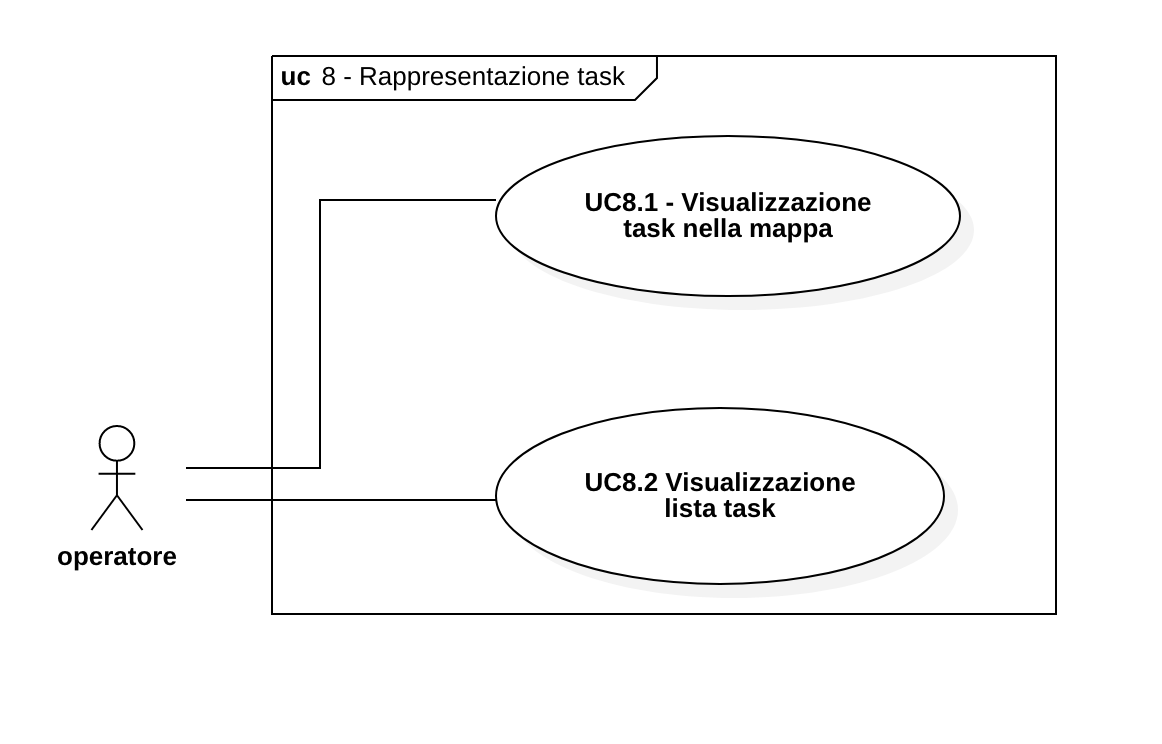
\includegraphics[scale=0.52]{res/images/uc8.png}
	\caption{UC8 - Rappresentazione task}
\end{figure}


\begin{itemize}
	\item 	\textbf{Attori primari:} operatore;
	\item 	\textbf{Precondizioni:} l'operatore si appresta a svolgere i propri compiti;
	\item 	\textbf{Postcondizioni:} l'operatore ha una visione completa dei suoi compiti tramite la mappa con i POI interessati e la lista completa di task da eseguire;
	\item 	\textbf{Scenario principale:} il sistema rende disponibile la visualizzazione di tutte le task assegnate all'operatore; essa avviene tramite la mappa con i POI di interesse per l'operatore e sottostante la lista di tutte le task con le relative informazioni;
	\item 	\textbf{Descrizione:} per compiere il suo lavoro, l'operatore ha bisogno di visualizzare le task che gli sono assegnate e la loro posizione, così da poter scaricare la merce nel luogo corretto.

\end{itemize}

\subsubsection{UC8.1 - Visualizzazione task nella mappa}
\begin{itemize}
	\item 	\textbf{Attori primari:} operatore;
	\item 	\textbf{Precondizioni:} l'operatore si appresta a svolgere i propri compiti;
	\item 	\textbf{Postcondizioni:} vengono visualizzate nella mappa le task nella relativa posizione, il prossimo POI che deve raggiungere per completare la task sarà evidenziato con un colore diverso;
	\item 	\textbf{Scenario principale:} l'operatore visualizza la mappa del magazzino. Sono rappresentati graficamente i POI relativi alle task assegnate, inoltre il prossimo da raggiungere sarà evidenziato con un colore diverso;
	\item 	\textbf{Descrizione:} per capire dove si trovano nel magazzino i punti da raggiungere per soddisfare le proprie task\textsubscript{G}, l'operatore deve avere una visione della mappa e dei POI che gli interessano. Inoltre deve essere ben visibile il prossimo POI che deve raggiungere per completare il prossimo compito che intende intraprendere.
\end{itemize}



\subsubsection{UC8.2 - Visualizzazione lista di task}
\begin{itemize}
	\item 	\textbf{Attori primari:} operatore;
	\item 	\textbf{Precondizioni:} l'operatore si appresta a svolgere i propri compiti;
	\item 	\textbf{Postcondizioni:} viene visualizzata una lista di tutte le task da eseguire con l'informazione sul relativo POI di scarico;
	\item 	\textbf{Scenario principale:} sotto alla mappa del magazzino, viene visualizzata una lista di tutte le task che l'operatore deve soddisfare. Ognuna mostra anche il codice identificativo del relativo POI di scarico;
	\item 	\textbf{Descrizione:} viene visualizzata la lista di task da completare da l'operatore.
\end{itemize}

\subsection{UC9 - Segnalazione del completamento di una task}
\begin{itemize}
	\item 	\textbf{Attori primari:} operatore;
	\item 	\textbf{Precondizioni:} l'operatore ha raggiunto il POI di scarico interessato per il completamento di una task;
	\item 	\textbf{Postcondizioni:} il sistema ha registrato il completamento della task che verrà cancellata dalla lista completa di tutte le task da soddisfare e da quella personale dell'operatore;
	\item 	\textbf{Scenario principale:} appena l'operatore raggiunge il POI interessato, il sistema rende disponibile un bottone per segnalare il completamento della task. L'operatore lo prene non appena ha finito di scaricare la merce ed è pronto a ripartire;
	\item 	\textbf{Descrizione:} l'operatore ha scaricato la merce nel punto destinato, quindi deve segnalare di aver completato la task per poter proseguire con la prossima.

\end{itemize}

\subsection{UC10 - Visualizzazione spostamenti del pilota automatico}
\begin{itemize}
	\item 	\textbf{Attori primari:} operatore;
	\item 	\textbf{Precondizioni:} è attiva la guida automatica del muletto;
	\item 	\textbf{Postcondizioni:} l'operatore visualizza la direzione degli spostamenti del pilota automatico;
	\item 	\textbf{Scenario principale:} il sistema controlla il movimento dell'unità e visualizza i cambi di direzione; nella mappa visualizza il proprio muletto effettuare lo spostamento;
	\item 	\textbf{Descrizione:} le unità possono essere guidate dal pilota automatico, ma gli spostamenti che il sistema ha intenzione di effettuare devono essere visualizzati dall'esterno.

\end{itemize}
 
\subsection{UC11 - Gestione guida}

\begin{figure}[H]
	\centering
	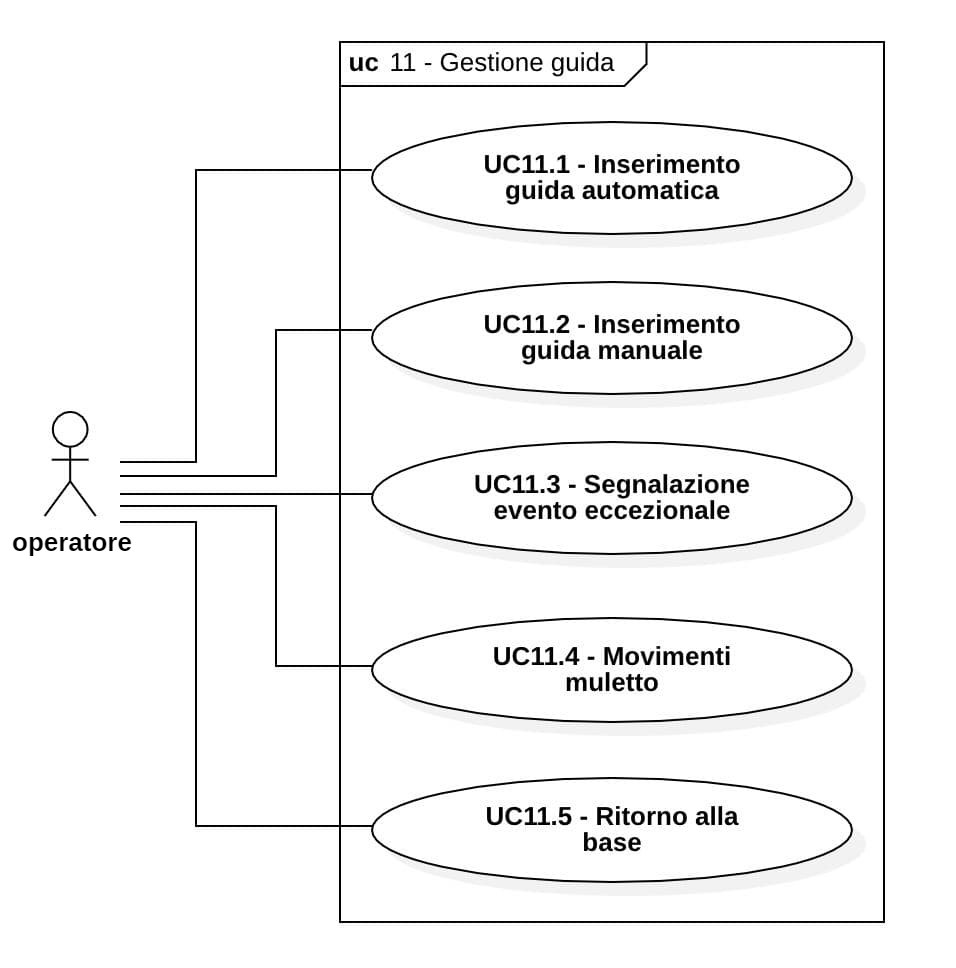
\includegraphics[scale=0.52]{res/images/uc11.png}
	\caption{ UC11 - Gestione guida}
\end{figure}

\begin{itemize}
	\item 	\textbf{Attori primari:} operatore;
	\item 	\textbf{Precondizioni:} l'operatore è pronto a svolgere il suo compito;
	\item 	\textbf{Postcondizioni:} l'operatore ha interagito correttamente con il sistema; 
	\item 	\textbf{Scenario principale:} l'operatore effettua le operazioni per la gestione della guida del muletto, ossia:
	\begin{itemize}
		\item l'inserimento della guida autonoma se è in modalità di guida manuale (UC11.1);
		\item l'inserimento della guida manuale se è in modalità di guida autonoma (UC11.2);
		\item la segnalazione di un evento eccezionale, per esempio ingorghi, collisioni o malfunzionamenti (UC11.3);
		\item lo spostamento del muletto all'interno della mappa (UC11.4);
	\end{itemize}
	\item 	\textbf{Descrizione:} l'operatore si appresta a guidare o a visualizzare le informazioni relative allo spostamento dell'unità. 

\end{itemize}

\subsubsection{UC11.1 - Inserimento guida automatica}
\begin{itemize}
	\item 	\textbf{Attori primari:} operatore;
	\item 	\textbf{Precondizioni:} la guida inserita è quella manuale;
	\item 	\textbf{Postcondizioni:} il sistema controlla il movimento del muletto;
	\item 	\textbf{Scenario principale:} l'operatore preme il pulsante apposito per il passaggio a guida automatica; il sistema cambia lo stato di guida e pilota autonomamente l'unità;
	\item 	\textbf{Descrizione:} i muletti possono essere guidati sia in modo automatico dal sistema che manuale, in base alle esigenze dell'operatore.
\end{itemize}

\subsubsection{UC11.2 - Inserimento guida manuale}
\begin{itemize}
	\item 	\textbf{Attori primari:} operatore;
	\item 	\textbf{Precondizioni:} il sistema centrale controlla il movimento del muletto;
	\item 	\textbf{Postcondizioni:} l'operatore guida il muletto manualmente; 
	\item 	\textbf{Scenario principale:} l'operatore preme il pulsante apposito per il passaggio a guida manuale; il sistema rende disponibile l'interfaccia per guidare l'unità;
	\item 	\textbf{Descrizione:} i muletti possono essere guidati sia in modo automatico dal sistema che manuale, in base alle esigenze dell'operatore.
\end{itemize}

\subsubsection{UC11.3 - Segnalazione evento eccezionale}
\begin{itemize}
	\item 	\textbf{Attori primari:} operatore;
	\item 	\textbf{Precondizioni:} il muletto si sta muovendo all'interno della mappa;
	\item 	\textbf{Postcondizioni:} un evento eccezionale è stato segnalato al sistema centrale; 
	\item 	\textbf{Scenario principale:} l'operatore preme il pulsante apposito per la segnalazione di un evento eccezionale; il sistema riceve l'informazione che viene visualizzata dall'amministratore;
	\item 	\textbf{Descrizione:} durante la guida possono verificarsi degli eventi eccezionali per esempio collisioni, ingorghi o malfunzionamenti del muletto. L'operatore deve segnalarli e il sistema centrale ha il compito di propagarli all'amministratore affinché possano essere gestiti.

\end{itemize}

\subsubsection{UC11.4 - Movimenti muletto}

\begin{figure}[H]
	\centering
	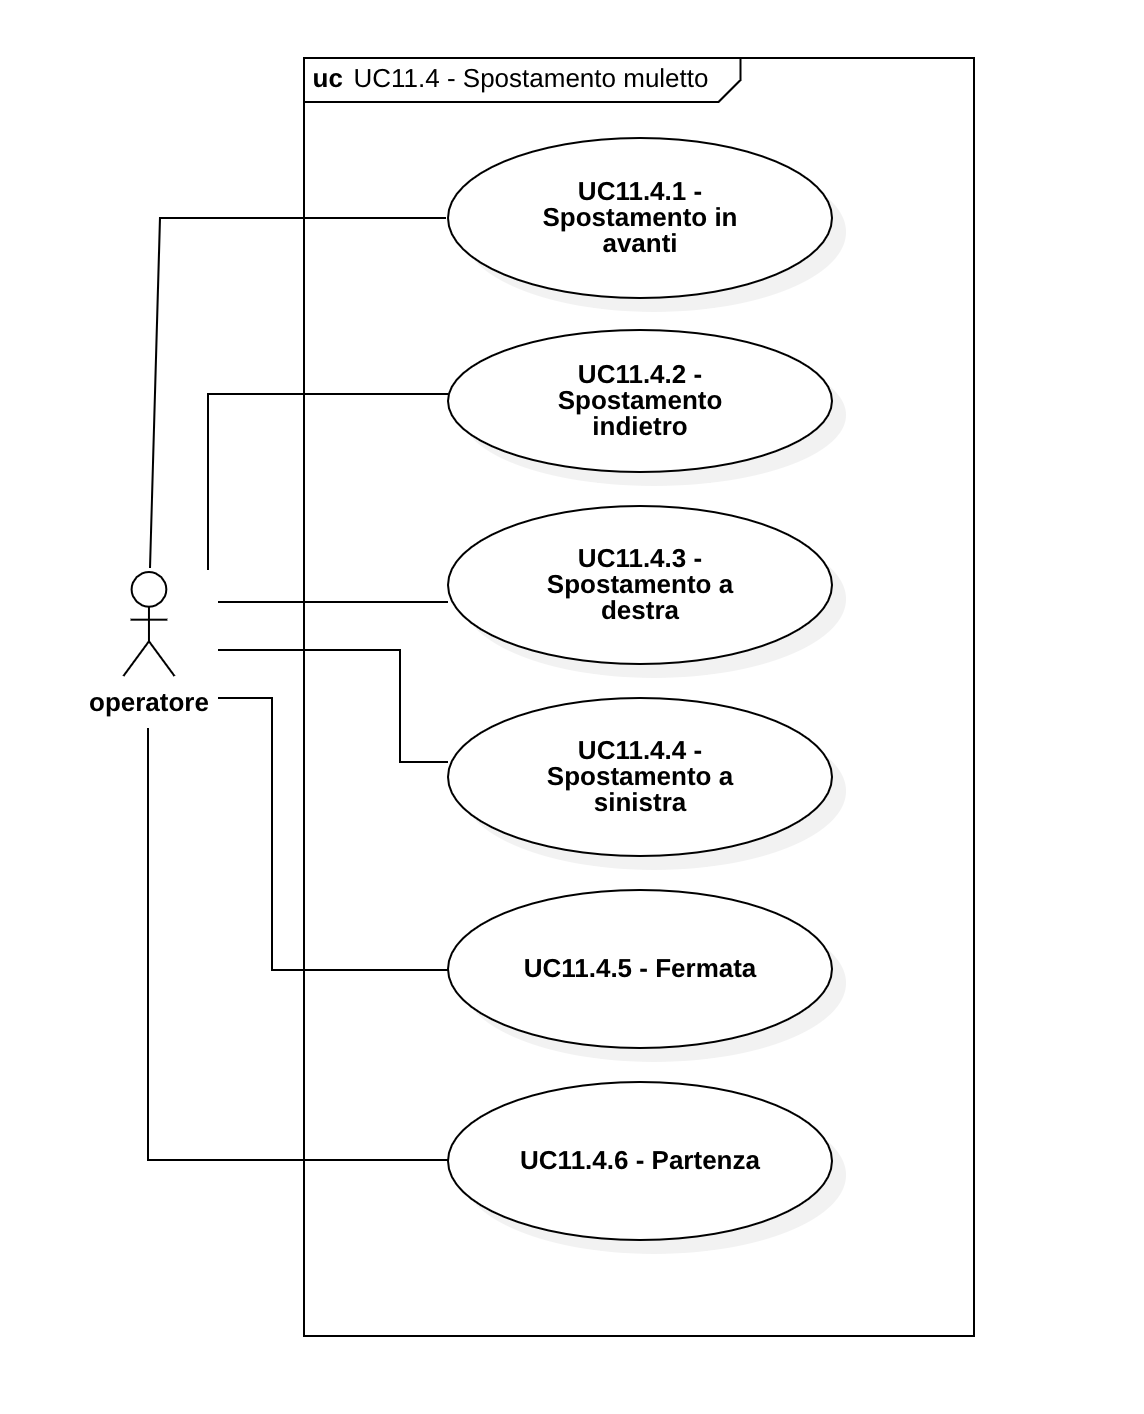
\includegraphics[scale=0.52]{res/images/uc11-4.png}
	\caption{UC11.4 - Movimenti muletto}
\end{figure}

\begin{itemize}
	\item 	\textbf{Attori primari:} operatore;
	\item 	\textbf{Precondizioni:} la modalità di guida è quella manuale;
	\item 	\textbf{Postcondizioni:} il muletto ha effettuato un movimento;
	\item 	\textbf{Scenario principale:} il sistema rende disponibile l'interfaccia per i movimenti del muletto, ossia le quattro frecce direzionali e un pulsante di start/stop. L'operatore può eseguire le seguenti operazioni:
	\begin{itemize}
		\item rotazione di 180 gradi (UC1.4.1);
		\item rotazione di 90 gradi in senso orario (UC1.4.2);
		\item rotazione di 90 gradi in senso antiorario (UC1.4.3);
		\item fermata (UC1.4.4);
		\item partenza (UC1.4.5);
	\end{itemize}
	\item 	\textbf{Descrizione:} i muletti possono intraprendere degli spostamenti all'interno della mappa per raggiungere i vari POI. Essi possono essere controllati manualmente dall'operatore.
\end{itemize}


\paragraph{UC11.4.1 - Rotazione di 180 gradi}
\begin{itemize}
	\item 	\textbf{Attori primari:} operatore;
	\item 	\textbf{Precondizioni:} l'operatore controlla il movimento del muletto;
	\item 	\textbf{Postcondizioni:} il muletto ha effettuato una rotazione di 180 gradi; 
	\item 	\textbf{Scenario principale:} l'operatore preme il pulsante apposito per la rotazione dell'unità di 180 gradi; il sistema riceva lo spostamento; il muletto nell'interfaccia dell'operatore viene girato;
	\item 	\textbf{Descrizione:} l'operatore intende invertire la rotta del muletto, rispetto alla propria direzione, all'interno della mappa.
\end{itemize}

\paragraph{UC11.4.2 - Rotazione di 90 gradi in senso orario}
\begin{itemize}
	\item 	\textbf{Attori primari:} operatore;
	\item 	\textbf{Precondizioni:} l'operatore controlla il movimento del muletto;
	\item 	\textbf{Postcondizioni:} il muletto ha effettuato rotazione di 90 gradi in senso orario; 
	\item 	\textbf{Scenario principale:} l'operatore preme il pulsante apposito per la rotazione dell'unità di 90 gradi in senso orario; l'unità effettua la rotazione;
	\item 	\textbf{Descrizione:} l'operatore intende far fare al muletto una rotazione di 90 gradi in senso orario, rispetto alla propria direzione, all'interno della mappa.
\end{itemize}

\paragraph{UC11.4.3 - Rotazione di 90 gradi in senso antiorario}
\begin{itemize}
	\item 	\textbf{Attori primari:} operatore;
	\item 	\textbf{Precondizioni:} l'operatore controlla il movimento del muletto;
	\item 	\textbf{Postcondizioni:} il muletto ha effettuato rotazione di 90 gradi in senso antiorario; 
	\item 	\textbf{Scenario principale:} l'operatore preme il pulsante apposito per la rotazione dell'unità di 90 gradi in senso antiorario; l'unità effettua la rotazione;
	\item 	\textbf{Descrizione:} l'operatore intende far fare al muletto una rotazione di 90 gradi in senso antiorario, rispetto alla propria direzione, all'interno della mappa.
\end{itemize}


\paragraph{UC11.4.5 - Fermata}
\begin{itemize}
	\item 	\textbf{Attori primari:} operatore;
	\item 	\textbf{Precondizioni:} l'operatore controlla il movimento del muletto, esso è in azione e si sta muovendo; Il sistema rende disponibile il pulsante di stop;
	\item 	\textbf{Postcondizioni:} il muletto è fermo all'interno della mappa o in base;
	\item 	\textbf{Scenario principale:} l'operatore preme il pulsante di stop; l'unità si ferma;
	\item 	\textbf{Descrizione:} quando il muletto è in movimento è possibile fermarne il moto. Per ripartire sarà necessario azionare il pulsante di partenza (UC11.4.5).
\end{itemize}


\paragraph{UC11.4.6 - Partenza}
\begin{itemize}
	\item 	\textbf{Attori primari:} operatore;
	\item 	\textbf{Precondizioni:} l'operatore controlla il movimento del muletto, esso è stato precedentemente fermato (UC11.4.5) oppure si trova alla base pronto per iniziare a lavorare; il sistema rende disponibile il pulsante di start;
	\item 	\textbf{Postcondizioni:} il muletto è in azione;
	\item 	\textbf{Scenario principale:} l'operatore preme il pulsante di start;
	\item 	\textbf{Descrizione:} il muletto deve essere azionato affinché l'unità parta:
	\begin{itemize}
		\item dalla base per raggiungere i POI da soddisfare;
		\item dopo aver effettuato una fermata a causa di un imprevisto o dello scarico delle merci (UC11.4.5).
	\end{itemize}
\end{itemize}


\subsubsection{UC11.5 - Ritorno alla base}
\begin{itemize}
	\item 	\textbf{Attori primari:} operatore;
	\item 	\textbf{Precondizioni:} l'operatore ha finito il turno e ha eseguito tutte le task assegnatoli. Il sistema rende disponibile un pulsante per il ritorno alla base;
	\item 	\textbf{Postcondizioni:} il muletto è nel punto della mappa base;
	\item 	\textbf{Scenario principale:} l'operatore preme nell'apposito pulsante per il ritorno alla base. Se la guida è impostata in manuale dovrà guidare fino al punto, altrimenti il sistema lo porta a destinazione;
	\item 	\textbf{Descrizione:} quando ha finito il turno, l'operatore deve ritornare alla base dove lascia il proprio mezzo per essere usato da un altro operatore.
\end{itemize}

\subsection{UC12 - Visualizzazione lista completa di POI}
\begin{itemize}
	\item 	\textbf{Attori primari:} amministratore, responsabile;
	\item 	\textbf{Precondizioni:} gli utenti sono autenticati;
	\item 	\textbf{Postcondizioni:} viene visualizzata la lista completa dei POI presenti nella mappa;
	\item 	\textbf{Scenario principale:} vicino alla visualizzazione della mappa (UC6), vi è un pulsante apposito per visualizzare la lista completa di POI presenti nel magazzino;
	\item 	\textbf{Descrizione:} per tener traccia di tutti i POI con il proprio tipo (carico, scarico, base) presenti nella mappa, il sistema rende disponibile la lista.

\end{itemize}

\subsection{UC13 - Visualizzazione liste ordinate di task}

\begin{figure}[H]
	\centering
	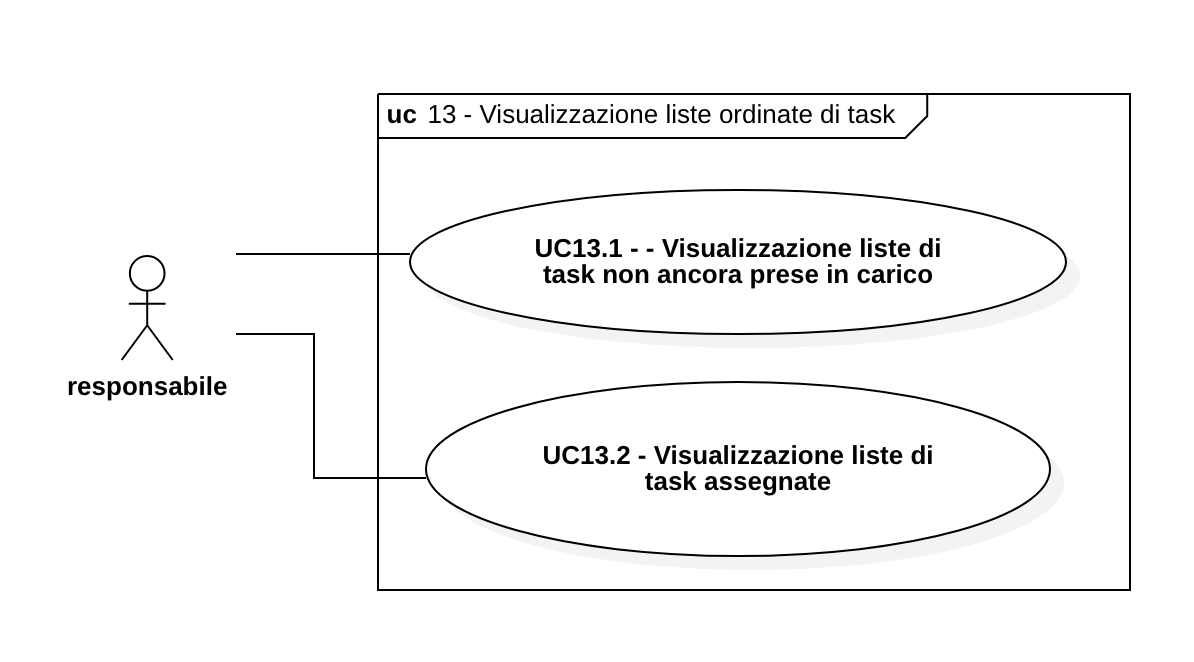
\includegraphics[scale=0.52]{res/images/uc13.png}
	\caption{UC13 - Visualizzazione liste ordinate di task}
\end{figure}

\begin{itemize}
	\item 	\textbf{Attori primari:} responsabile;
	\item 	\textbf{Precondizioni:} l'utente è autenticato come utente responsabile;
	\item 	\textbf{Postcondizioni:} il responsabile visualizza l'insieme di liste ordinate di task;
	\item 	\textbf{Scenario principale:} nell'interfaccia utente del responsabile, viene visualizzato l'insieme di liste ordinate di task, divise per liste già assegnate ad un'unità e quelle non ancora prese in carico, che possono ancora venire modificate;
	\item 	\textbf{Descrizione:} la task sono inserite dal responsabile in liste, ognuna delle quali viene assegnata dal sistema ad un'unità per essere completata. Il responsabile necessita di poter visualizzare l'insieme delle task per tenere sotto controllo l'andamento del magazzino.

\end{itemize}

\subsubsection{UC13.1 - Visualizzazione liste di task non ancora prese in carico}
\begin{itemize}
	\item 	\textbf{Attori primari:} responsabile;
	\item 	\textbf{Precondizioni:} l'utente è autenticato come utente responsabile;
	\item 	\textbf{Postcondizioni:} il responsabile visualizza l'insieme delle liste delle task non ancora prese in carico dalle unità;
	\item 	\textbf{Scenario principale:} il responsabile visualizza vicino alla mappa (UC6.1) un elenco delle liste delle task non ancora assegnate dal sistema alle unità per essere soddisfatte;
	\item 	\textbf{Descrizione:} la task sono inserite dal responsabile in liste, ognuna delle quali viene assegnata dal sistema ad un'unità per essere completata. Il responsabile necessità di poter visualizzare l'insieme delle task non ancora prese in carico per controllare quanto lavoro manca da completare.


\end{itemize}

\subsubsection{UC13.2 - Visualizzazione liste di task assegnate}
\begin{itemize}
	\item 	\textbf{Attori primari:} responsabile;
	\item 	\textbf{Precondizioni:} l'utente è autenticato come utente responsabile;
	\item 	\textbf{Postcondizioni:} il responsabile visualizza l'insieme delle liste delle task assegnate a delle unità;
	\item 	\textbf{Scenario principale:} il responsabile visualizza vicino alla mappa (UC6.1), un elenco delle liste di task con la relativa unità alla quale ogni lista è assegnata. Inoltre queste liste si aggiorneranno al soddisfacimento di una task per visualizzare solo la successiva;
	\item 	\textbf{Descrizione:} la task sono inserite dal responsabile in liste, ognuna delle quali viene assegnata dal sistema ad un'unità per essere completata. Il responsabile necessità di poter visualizzare l'insieme di task già assegnate e il loro andamento.

\end{itemize}

\subsection{UC14 - Gestione unità}

\begin{figure}[H]
	\centering
	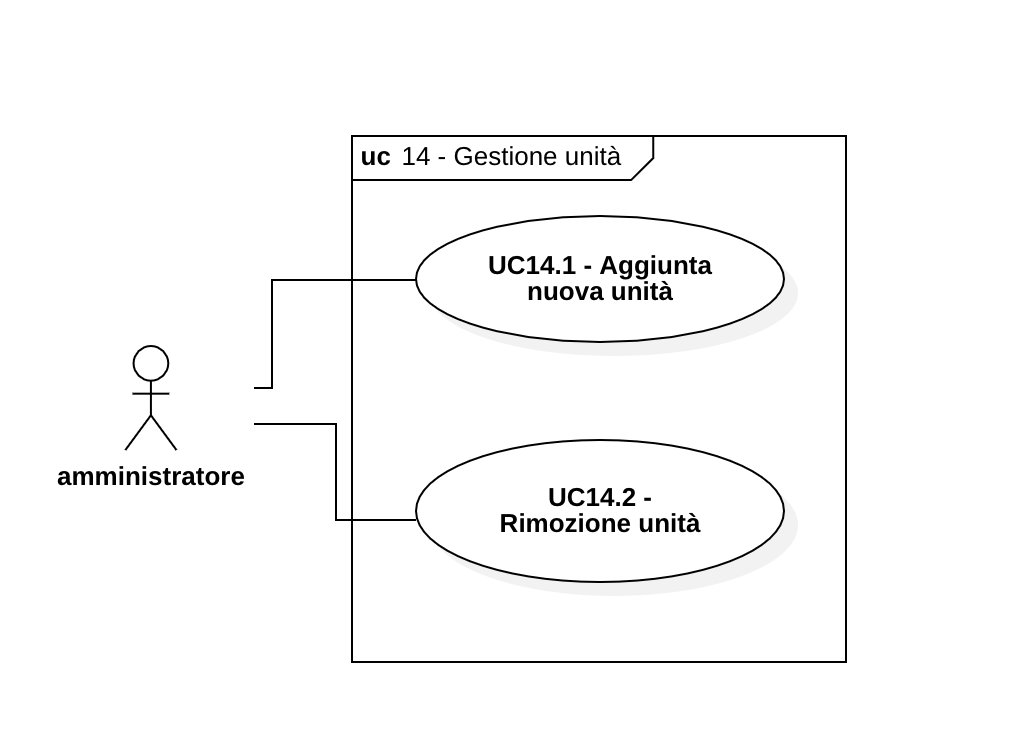
\includegraphics[scale=0.52]{res/images/uc14.png}
	\caption{UC14 - Gestione unità}
\end{figure}

\begin{itemize}
	\item 	\textbf{Attori primari:} amministratore;
	\item 	\textbf{Precondizioni:} l'utente è autenticato come amministratore e viene resa disponibile l'interfaccia per la gestione delle unità;
	\item 	\textbf{Postcondizioni:} è cambiata la quantità di unità gestite dal sistema;
	\item 	\textbf{Scenario principale:} l'amministratore dopo aver premuto il pulsante per la gestione delle unità, visualizza le operazioni che può effettuare:
	\begin{itemize}
		\item l'aggiunta di un nuovo mezzo (UC14.1);
		\item la rimozione di un mezzo esistente (UC14.2);
	\end{itemize}
	\item 	\textbf{Descrizione:} ogni unità (muletto) deve essere identificata all'interno del magazzino attraverso il proprio codice identificativo. L'amministratore ha il compito di gestire l'aggiunta di un nuovo muletto all'interno del magazzino e la sua eliminazione.
\end{itemize}

\subsubsection{UC14.1 - Aggiunta nuova unità}
\begin{itemize}
	\item 	\textbf{Attori primari:} amministratore;
	\item 	\textbf{Precondizioni:} l'amministratore sta visualizzando l'interfaccia per l'aggiunta di un nuovo mezzo;
	\item 	\textbf{Postcondizioni:} è stata aggiunta un'unità all'interno del sistema con il relativo codice identificativo;
	\item 	\textbf{Scenario principale:} l'amministratore visualizza un form per l'inserimento del codice identificativo del muletto e conferma l'aggiunta.
	\item 	\textbf{Descrizione:} quando viene utilizzato un nuovo muletto all'interno del magazzino, esso deve venire registrato nel sistema dall'amministratore assegnandogli un proprio codice identificativo.

\end{itemize}


\subsubsection{UC14.2 - Rimozione unità}
\begin{itemize}
	\item 	\textbf{Attori primari:} amministratore;
	\item 	\textbf{Precondizioni:} l'amministratore sta visualizzando l'interfaccia per la rimozione di un mezzo;
	\item 	\textbf{Postcondizioni:} un'unità è stata rimossa dal sistema;
	\item 	\textbf{Scenario principale:} l'amministratore seleziona l'unità che deve essere rimossa dal sistema e conferma la modifica;
	\item 	\textbf{Descrizione:} quando un muletto all'interno del magazzino non viene più utilizzato deve essere rimosso dal sistema.
	
\end{itemize}

\subsection{UC15 - Invio propria posizione}
\begin{itemize}
	\item 	\textbf{Attori primari:} unità;
	\item 	\textbf{Precondizioni:} l'unità si sta muovendo all'interno della mappa;
	\item 	\textbf{Postcondizioni:} la posizione nella mappa di una determinata unità è stata inviata al sistema centrale;
	\item 	\textbf{Scenario principale:} l'unità, ad ogni istante t, invia le coordinate della propria posizione e la sua direzione;
	\item 	\textbf{Descrizione:} ad ogni istante di tempo t, il server deve conoscere dove si trova esattamente ogni unità all'interno della mappa, così da poter gestire il movimento delle unità ed evitare collisioni.
	
\end{itemize}

\subsection{UC16 - Richiesta percorso fra due POI}
\begin{itemize}
	\item 	\textbf{Attori primari:} unità;
	\item 	\textbf{Precondizioni:} l'unità deve partire da un punto nella mappa per raggiungere il prossimo POI per soddisfare la successiva task nella sua lista;
	\item 	\textbf{Postcondizioni:} è stato ricevuto il percorso per raggiungere il prossimo POI;
	\item 	\textbf{Scenario principale:} l'unità una volta raggiunto un POI e soddisfatto la relativa task, richiede al sistema il percorso per raggiungere il prossimo punto di interesse in lista; tale percorso è un insieme di mosse che determinano gli spostamenti o il cambio di direzioni che l'unità dovrà intraprendere.
	\item 	\textbf{Descrizione:} il sistema calcola il percorso ottimale per raggiungere il prossimo POI per soddisfare la nuova task. Questo percorso deve essere inviato all'unità che effettuerà i movimenti descritti.
	
\end{itemize}

\subsection{UC17 - Modifica proprio account}

\begin{figure}[H]
	\centering
	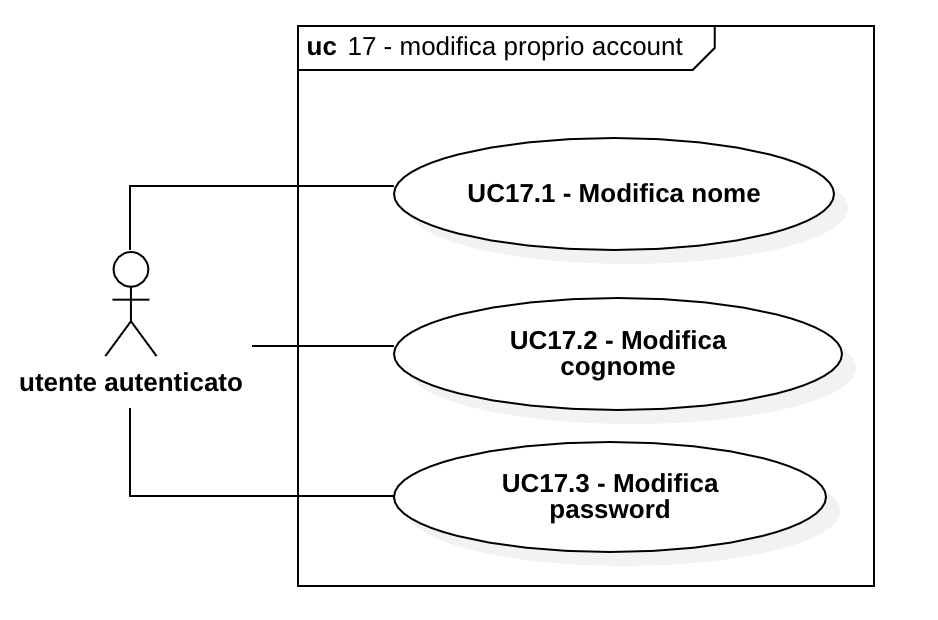
\includegraphics[scale=0.52]{res/images/uc17.png}
	\caption{UC17 - Modifica proprio account}
\end{figure}

\begin{itemize}
	\item 	\textbf{Attori primari:} utente autenticato;
	\item 	\textbf{Precondizioni:} l'utente è autenticato nel sistema;
	\item 	\textbf{Postcondizioni:} viene cambiato il profilo dell'utente;
	\item 	\textbf{Scenario principale:} l'utente preme l'apposito pulsante per la modifica del proprio account. Il sistema rende disponibile l'interfaccia per la selezione del campo che si intende modificare:
	\begin{itemize}
		\item nome;
		\item cognome;
		\item password
	\end{itemize}
	A questo punto l'utente conferma le modifiche.
	\item 	\textbf{Descrizione:} l'utente modifica il proprio account personale.
\end{itemize}

\subsubsection{UC17.1 - Modifica nome}
\begin{itemize}
	\item 	\textbf{Attori primari:} utente autenticato;
	\item 	\textbf{Precondizioni:} l'utente è autenticato ha premuto il pulsante per la modifica account;
	\item 	\textbf{Postcondizioni:} viene cambiato il nome dell'utente;
	\item 	\textbf{Scenario principale:} l'utente modifica l'apposito form del proprio nome e conferma.
	\item 	\textbf{Descrizione:} l'utente modifica il proprio nome.
\end{itemize}

\subsubsection{UC17.2 - Modifica cognome}
\begin{itemize}
	\item 	\textbf{Attori primari:} utente autenticato;
	\item 	\textbf{Precondizioni:} l'utente è autenticato ha premuto il pulsante per la modifica account;
	\item 	\textbf{Postcondizioni:} viene cambiato il cognome dell'utente;
	\item 	\textbf{Scenario principale:} l'utente modifica l'apposito form del proprio cognome e conferma.
	\item 	\textbf{Descrizione:} l'utente modifica il proprio cognome.
\end{itemize}

\subsubsection{UC17.3 - Modifica password}
\begin{itemize}
	\item 	\textbf{Attori primari:} utente autenticato;
	\item 	\textbf{Precondizioni:} l'utente è autenticato ha premuto il pulsante per la modifica account;
	\item 	\textbf{Postcondizioni:} viene cambiato la password dell'utente;
	\item 	\textbf{Scenario principale:} l'utente modifica l'apposito form della propria password e conferma.
	\item 	\textbf{Descrizione:} l'utente modifica la propria password.
\end{itemize}